\input{common/macros/math.tex}
\input{common/macros/theorems.tex}
\usepackage[a4paper,hmargin=30mm,vmargin=30mm]{geometry}
\graphicspath{{./Cartes_postales/}{./Images/}}
\title{\color{astral} \sffamily \bfseries Paysage Mathématique: Cartes Postales}
\author{Stéphane Lejeune}
\date{\today}


\begin{document}
    \maketitle
    \tableofcontents

    \newpage
    
    \section{Introduction}\label{sec:s_1}

    \newpage
\section{Bateau}

\begin{figure}[h]
    \centering
    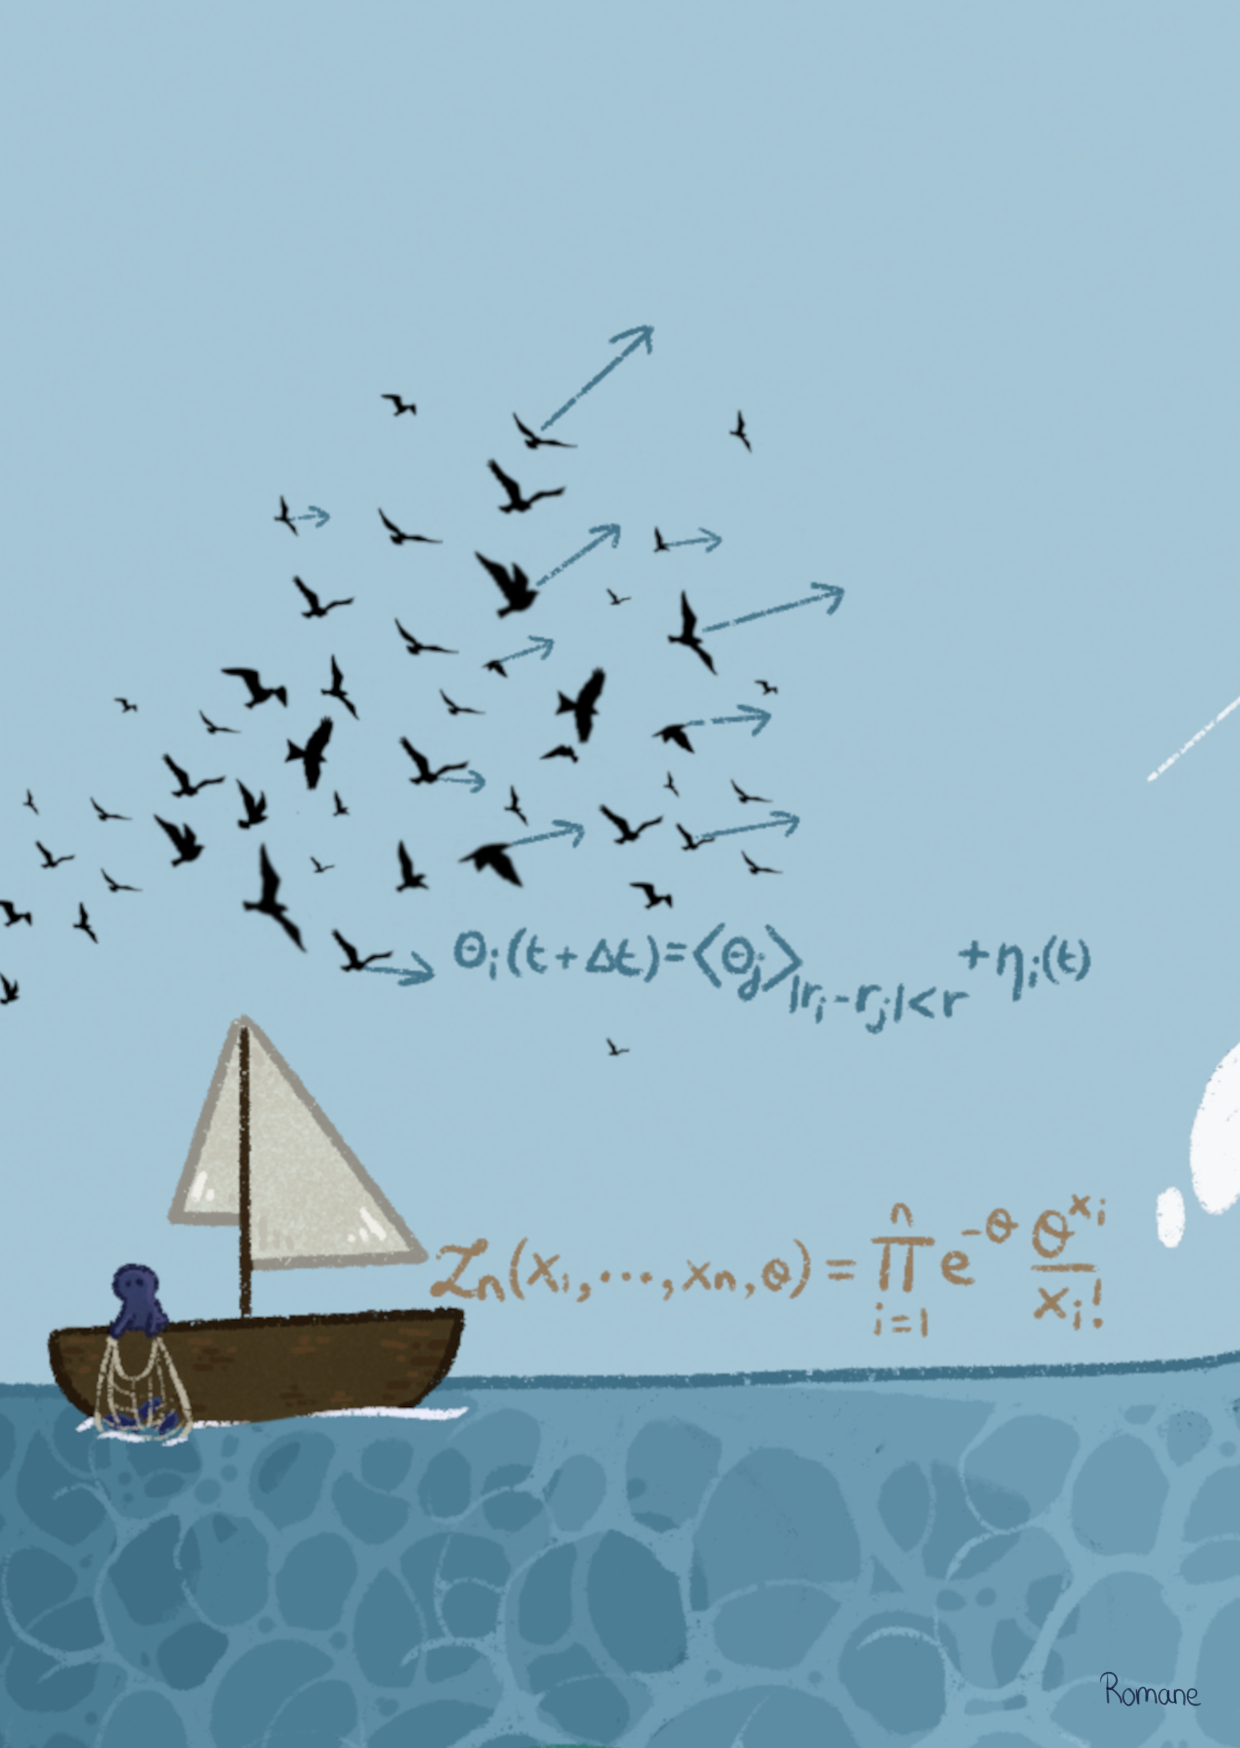
\includegraphics[height=0.5\textheight]{Cartes_postales/carte01-bateau.png}\label{fig:c1}
    \caption{Carte postale: Bateau}
\end{figure}

Sais-tu qu'on peut estimer le nombre de truites en mer? Pour cela, on utilise une méthode mathématique appelée capture-recapture. On commence par capturer des truites, on les marque et puis, on les relâche. Après un certain temps, on capture à nouveau des truites, c'est la recapture. On suppose que la proportion de truites marquées dans notre recapture parmi toutes les truites de notre recapture est la même proportion que celle de toutes les truites marquées parmi toutes les truites:

\begin{figure}[h]
    \centering
    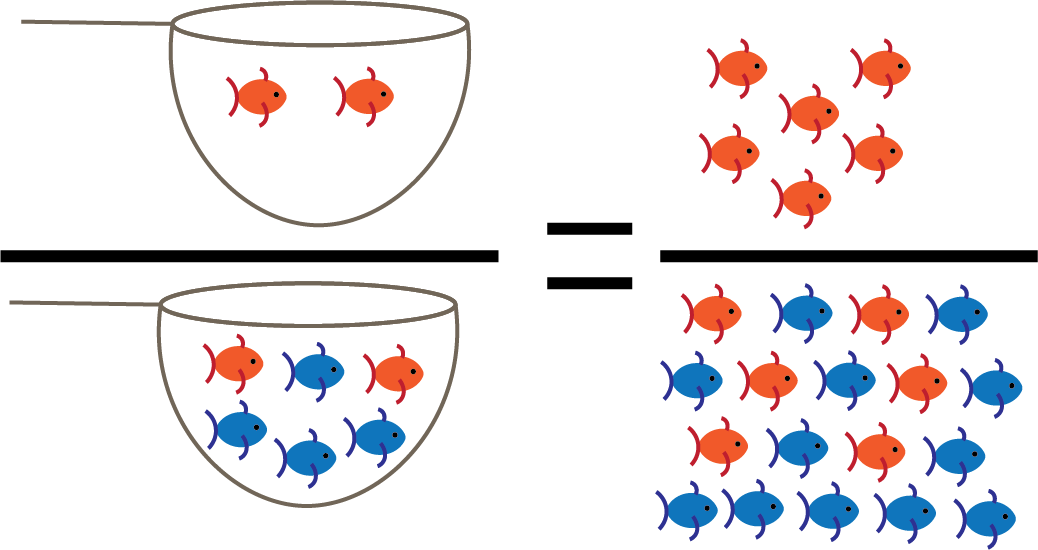
\includegraphics[height=0.1\textheight]{Images/poissons_v2.png}\label{fig:c1_poissons}
    \caption{Illustration de la formule}
\end{figure}

On peut en déduire une estimation du nombre total de truites en mer avec un produit en croix. En pratique, on utilise des méthodes plus poussées, toujours basées sur cette idée, car on rencontre beaucoup de problèmes liés au fait qu'on estime des populations d'êtres vivant, contrairement aux cours de maths où on compte des billes dans un sac. Voici quelques problèmes qu'on peut rencontrer: les marquages peuvent s'effacer, le nombre total de truites change, la population se dépace ailleurs. C'est pour ça qu'il y a beaucoup de recherches mathématique sur ces sujets.
    \newpage
\section{coquillage}

\begin{figure}[h]
    \centering
    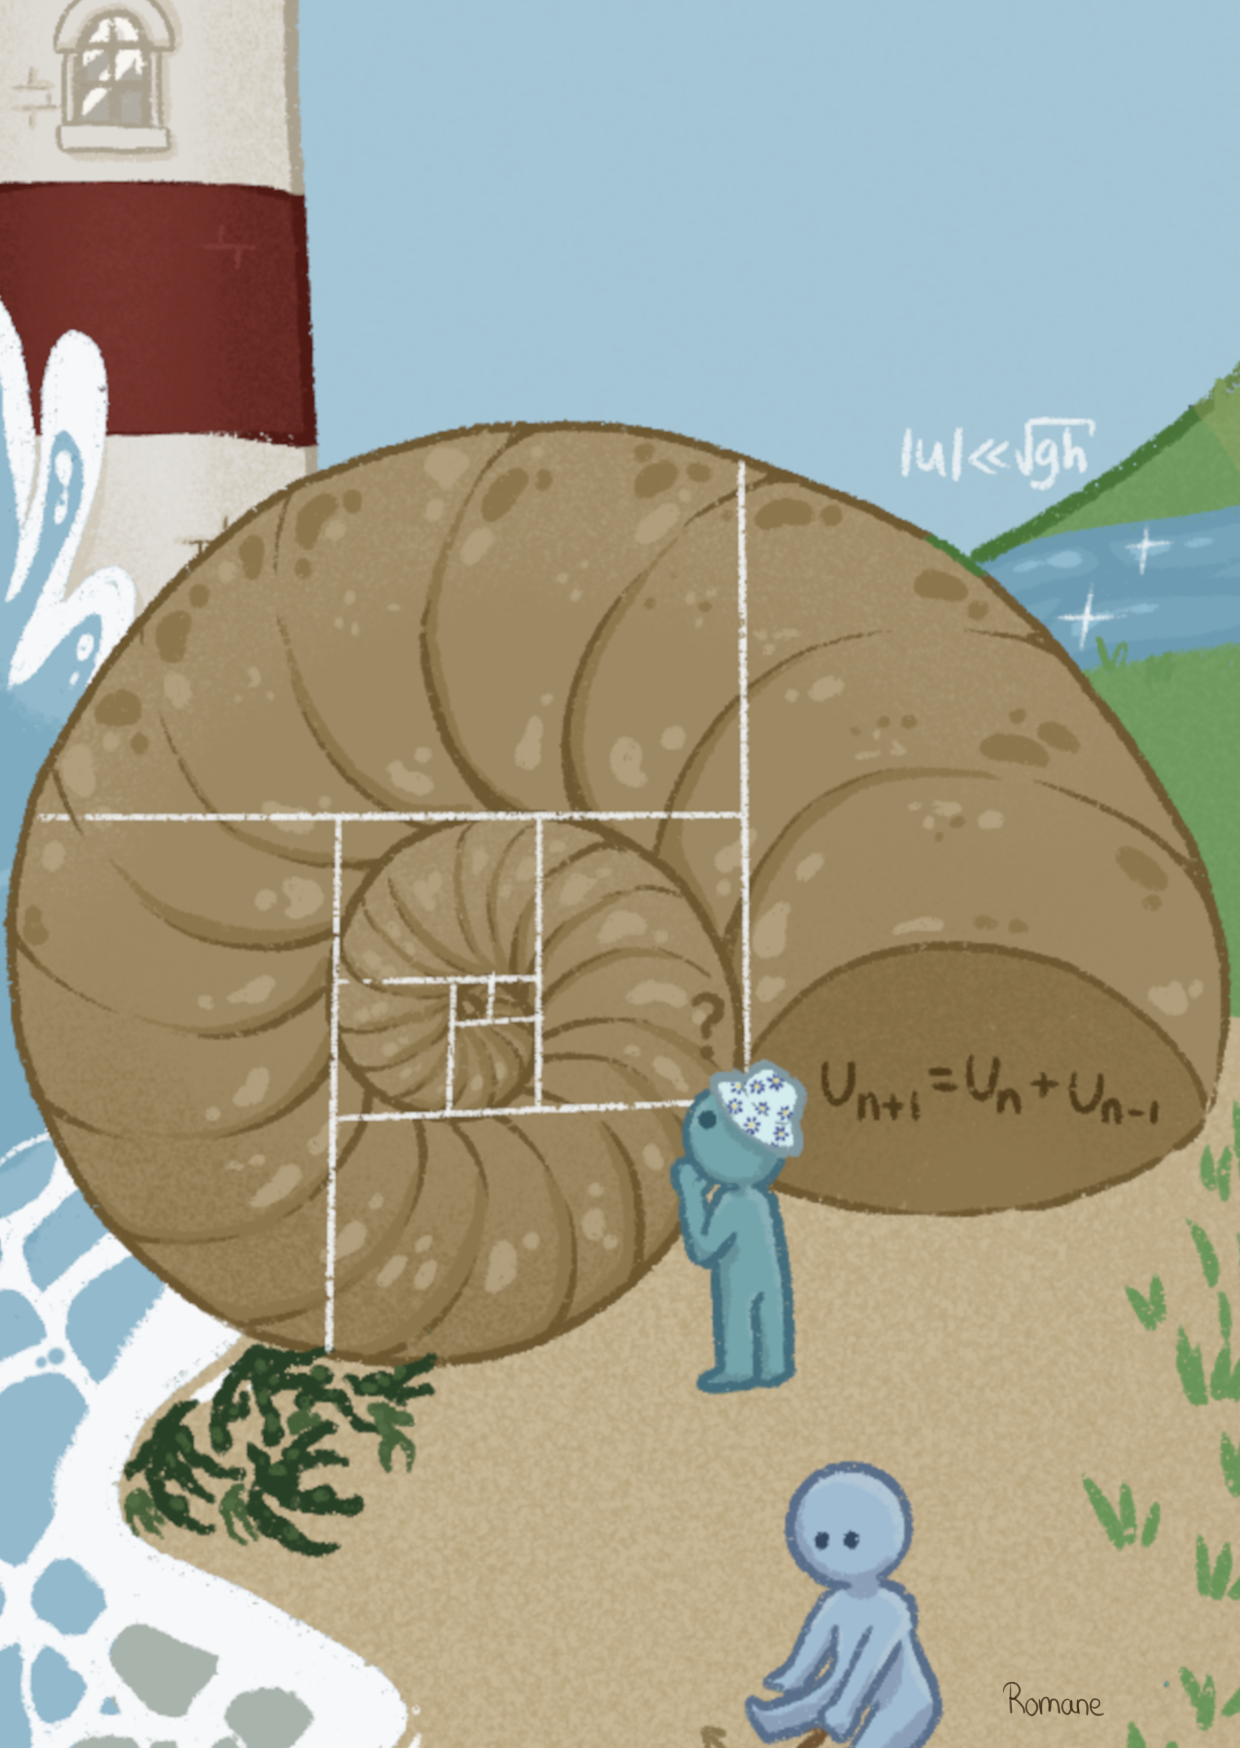
\includegraphics[height=0.5\textheight]{Cartes_postales/carte02-coquillage.png}\label{fig:c02}
    \caption{Carte postale: Coquillage}
\end{figure}

Les mathématiques nous aident à décrire les formes du vivant. Par exemple, le coquillage de la nautile a une forme de spirale logarithmique. La nautile crée sa coquille au fil de sa croissance, en l'élargissant et l'enroulant sur elle-même. Cette forme mathématique peut s'agrandir autant qu'on veuille en gardant exactement la même forme (plus précisément, cela revient à la tourner d'un certain angle). Si on zoom ou dézoom sur la spirale, on voit exactement la même chose, juste tourné un peu.

\medskip

Cette propriété est cruciale car elle permet aux nautilles de grandir sans devoir changer de forme ou créer une nouvelle maison tous les 3 mois. De plus, cette spirale est equiangle, la courbe s'éloigne du centre de manière très régulière, ce qui la rend très résistante à la pression. La pression se répartit uniformément sur tout le coquillage car il n'y a aucune partie plus fragile qui risque de céder en premier. Ceci lui permet de plonger très profondément mais aussi de resister à des prédateurs.


    \newpage
\section{Sable}

\begin{figure}[h]
    \centering
    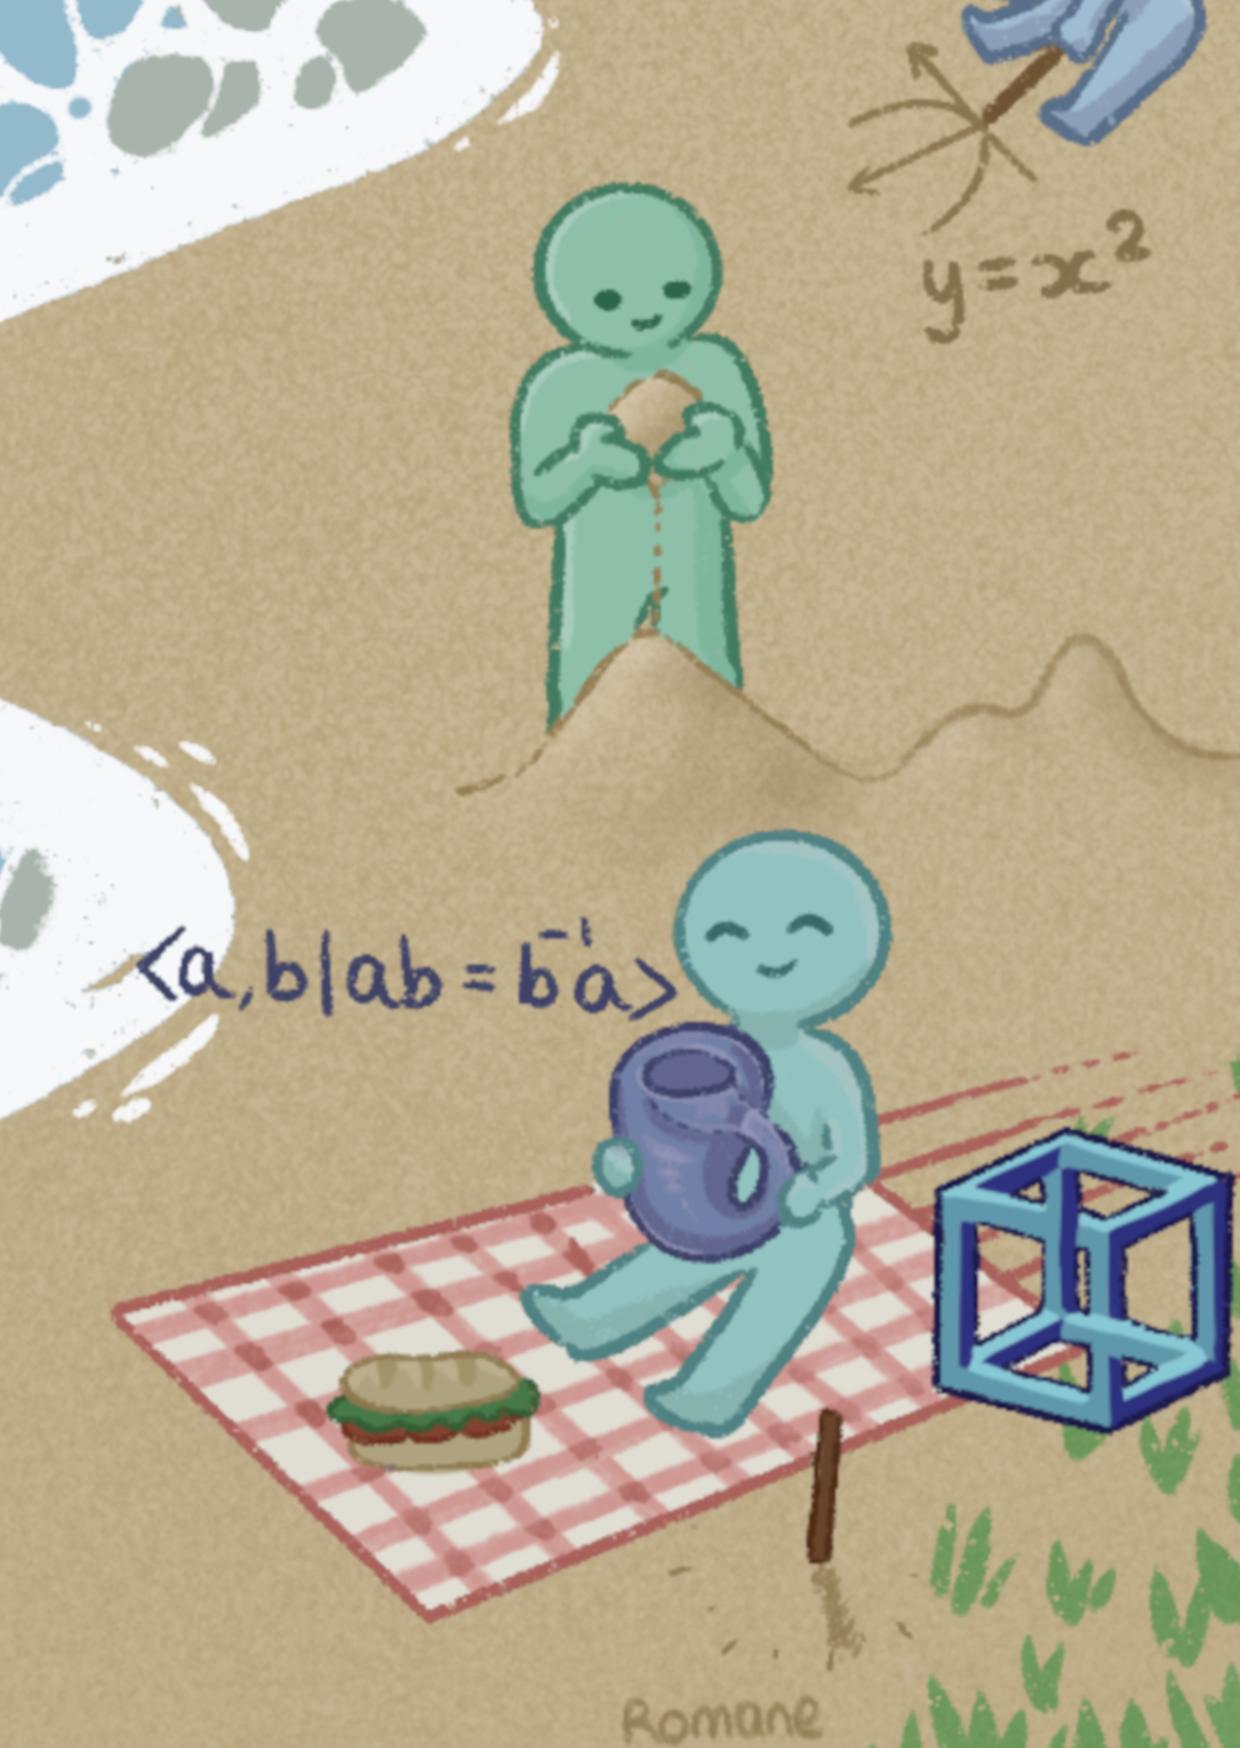
\includegraphics[height=0.5\textheight]{Cartes_postales/carte03-sable.png}\label{fig:c03}
    \caption{Carte postale: Sable}
\end{figure}

Les tas de sable ont des propriétés physique très intéressantes. Si on laisse tomber des grains de sable verticalement, on obtient un cône. Et l'angle au sommet de ce cône, appelé angle de repos, dépend à la fois de la gravité et des forces de frottements qui font que les grains de sable s'accrochent entre eux. En tombant, trois choses peuvent arriver: le tas de sable grossit, le grain déclenche un petit glissement, ou, très rarement, le grain déclenche une avalanche massive et une grande partie du tas s'effondre.

\medskip

On appelle ce genre de système un système critique: une petite variation locale peut entraîner des conséquences globales majeures. En mathématiques, on peut créer des modèles permettant de représenter ce genre de phénomène, et on peut estimer à quel point on est proche de ce seuil critique où une avalanche peut arriver. C'est très utile quand on part au ski!




    \newpage
\section{tournesol}

% \begin{figure}[h]
%     \centering
%     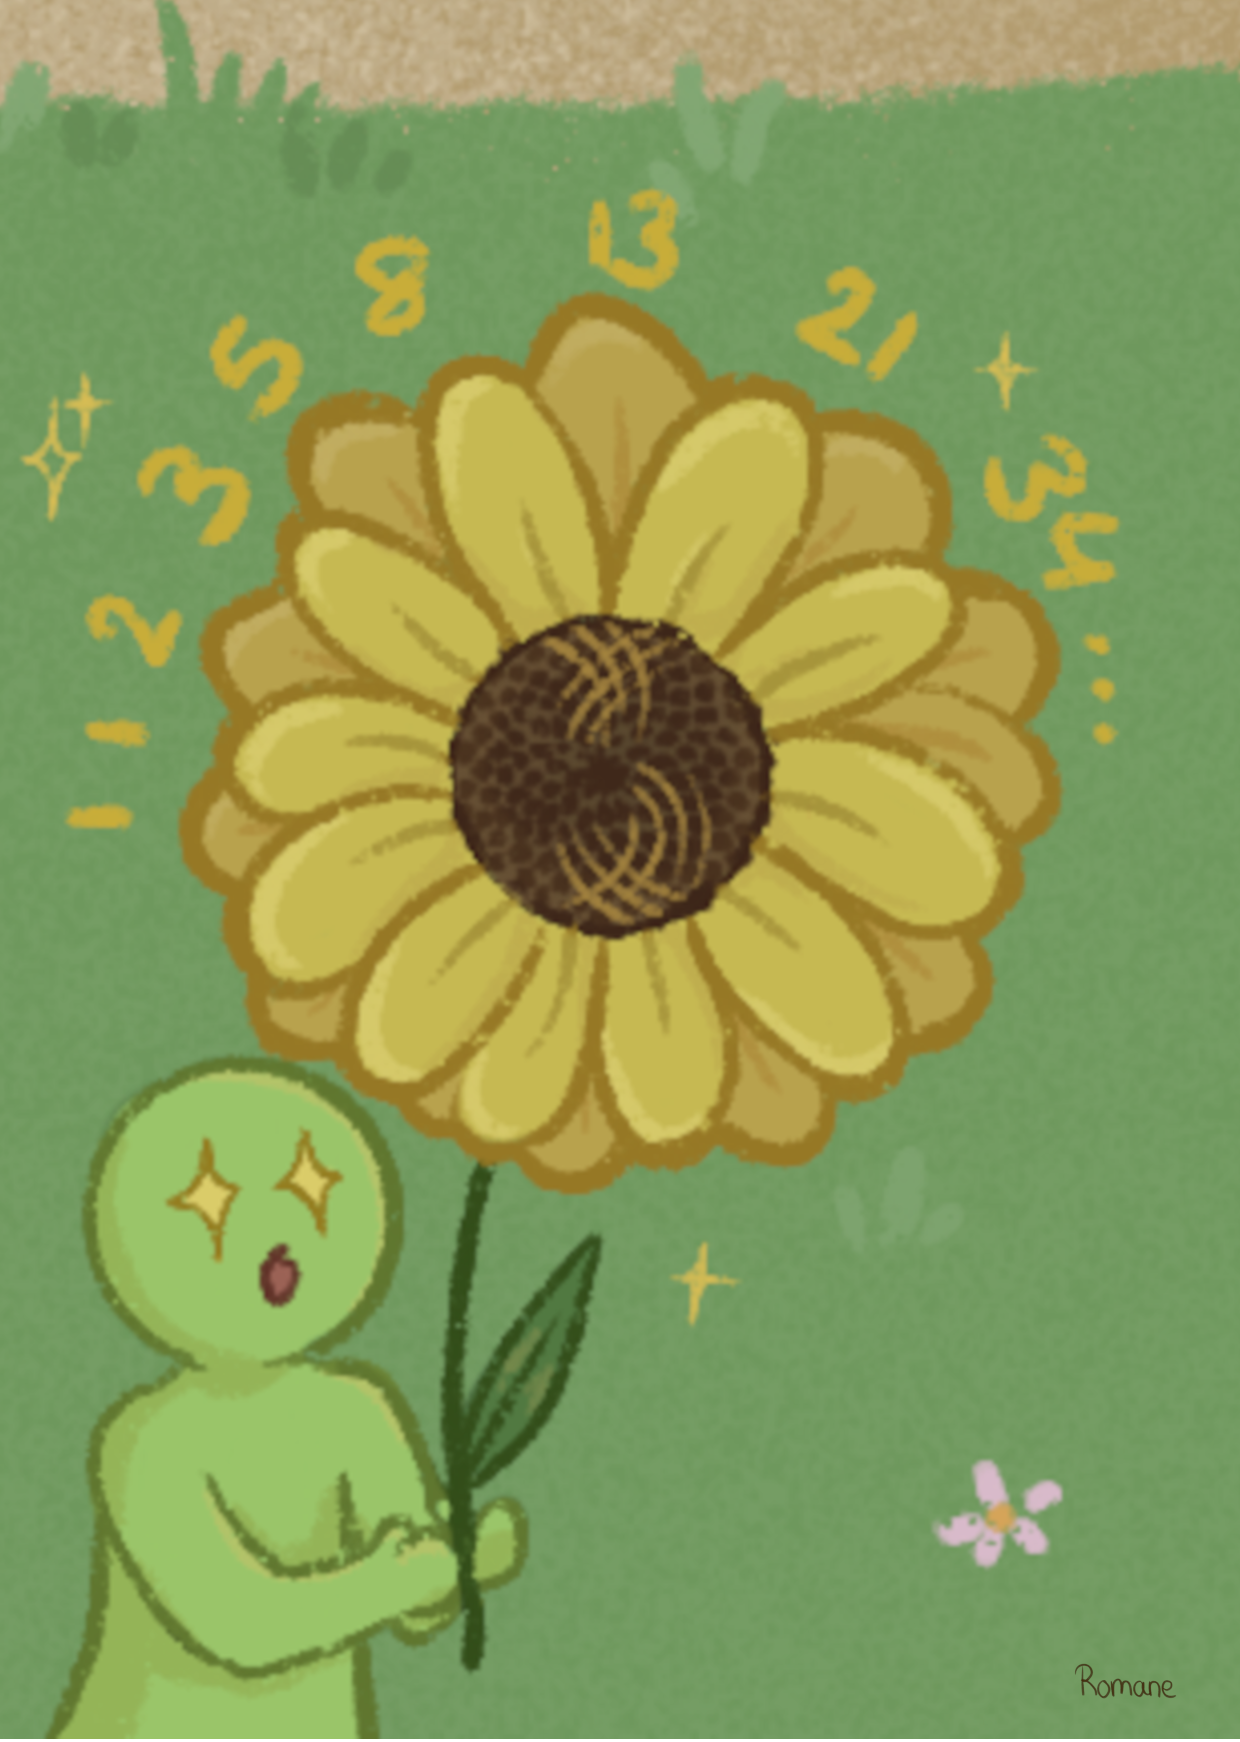
\includegraphics[height=0.5\textheight]{Cartes_postales/carte04-tournesol.png}\label{fig:c04}
%     \caption{Carte postale: Tournesol}
% \end{figure}

Les mathématiques permettent de décrire et comprendre la nature. La suite de Fibonacci est un exemple typique. C'est une suite de nombres définie de la manière suivante: les deux premiers nombres sont 0 et 1. Puis chaque nombre est obtenu en additionnant les deux précédents. Ainsi, les premiers nombres sont 0,1,1,2,3,5,8,13,21. Les termes de cette suite apparaissent dans de nombreux phénomènes de croissance dans le vivant, comme les graines de tournesol ou les formes de coquillages.

\begin{figure}[h]
    \centering
    \includegraphics[height=0.1\textheight]{Images/tournesol.png}\label{fig:c04_tournesol}
    \caption{Illustration pour différents angles}
\end{figure}

Les graines de tournesol grandissent en poussant les anciennes graines vers l'extérieur, et chaque nouvelle graine apparait depuis le centre en formant forment un angle avec les graines précédentes. Si l'angle est rationnel, par exemple 1/6, on aura 6 branches. Si l'angle vaut 11/23, on aura deux branches au début comme c'est une fraction proche de 1/2, puis on aura 23 branches. L'angle qui optimise l'espacement des graines est le nombre d'or, car c'est le plus irrationnel, et empêche les graines de s'aligner entre elles. Cet angle est très lié à la suite de Fibonnaci. On peut observer ces comportements dans le dessin ci-dessus.



\newpage
\subsection{Explications}

Les graines d'un tournesol apparaissent successivement à partir du centre de la fleur. Au fur et à mesure que les nouvelles graines apparaissent, elles repoussent les plus anciennes vers l'extérieur. Chaque nouvelle graine forme un angle avec la précédente, appelé angle de divergence. Afin de maximiser l'espacement des graines, il faut choisir un angle de divergence précis.

Si l'on choisit un angle rationnelle, par exemple un tiers de tour complet, la quatrième graine se retrouve dans l'axe de la première après trois itérations. En se poussant mutuellement, les graines finissent par former trois lignes droites. Cette structure est très inefficace car il y a beaucoup d'espace non utilisé. Ce phénomène se produit avec l'ensemble des nombres rationnels puisque, après un ou plusieurs tours complets (selon le numérateur), la structure se confronte à ce même problème d'alignement.

Il est donc plus avantageux pour la plante de prendre un nombre irrationnel comme l'angle de divergence. Pour éviter la formation de lignes, même légèrement courbées, on peut  choisir un nombre difficilement approximable par des fractions rationnelles. En mathématiques, le nombre le plus difficile à approcher par des nombres rationnels est le nombre d'or, en raison de son développement en fraction continue. C'est précisément cette proportion que l'on retrouve dans la construction des spirales de Fibonacci.

Avec cet angle spécifique, les graines ne forment jamais de lignes. Le développement des nouvelles graines engendre des spirales de Fibonacci et assure une répartition très homogène.

Image prise en utilisant https://sorciersdesalem.math.cnrs.fr/SpiralesFibo/spirale.html
    \newpage
\section{velo}

\begin{figure}[h]
    \centering
    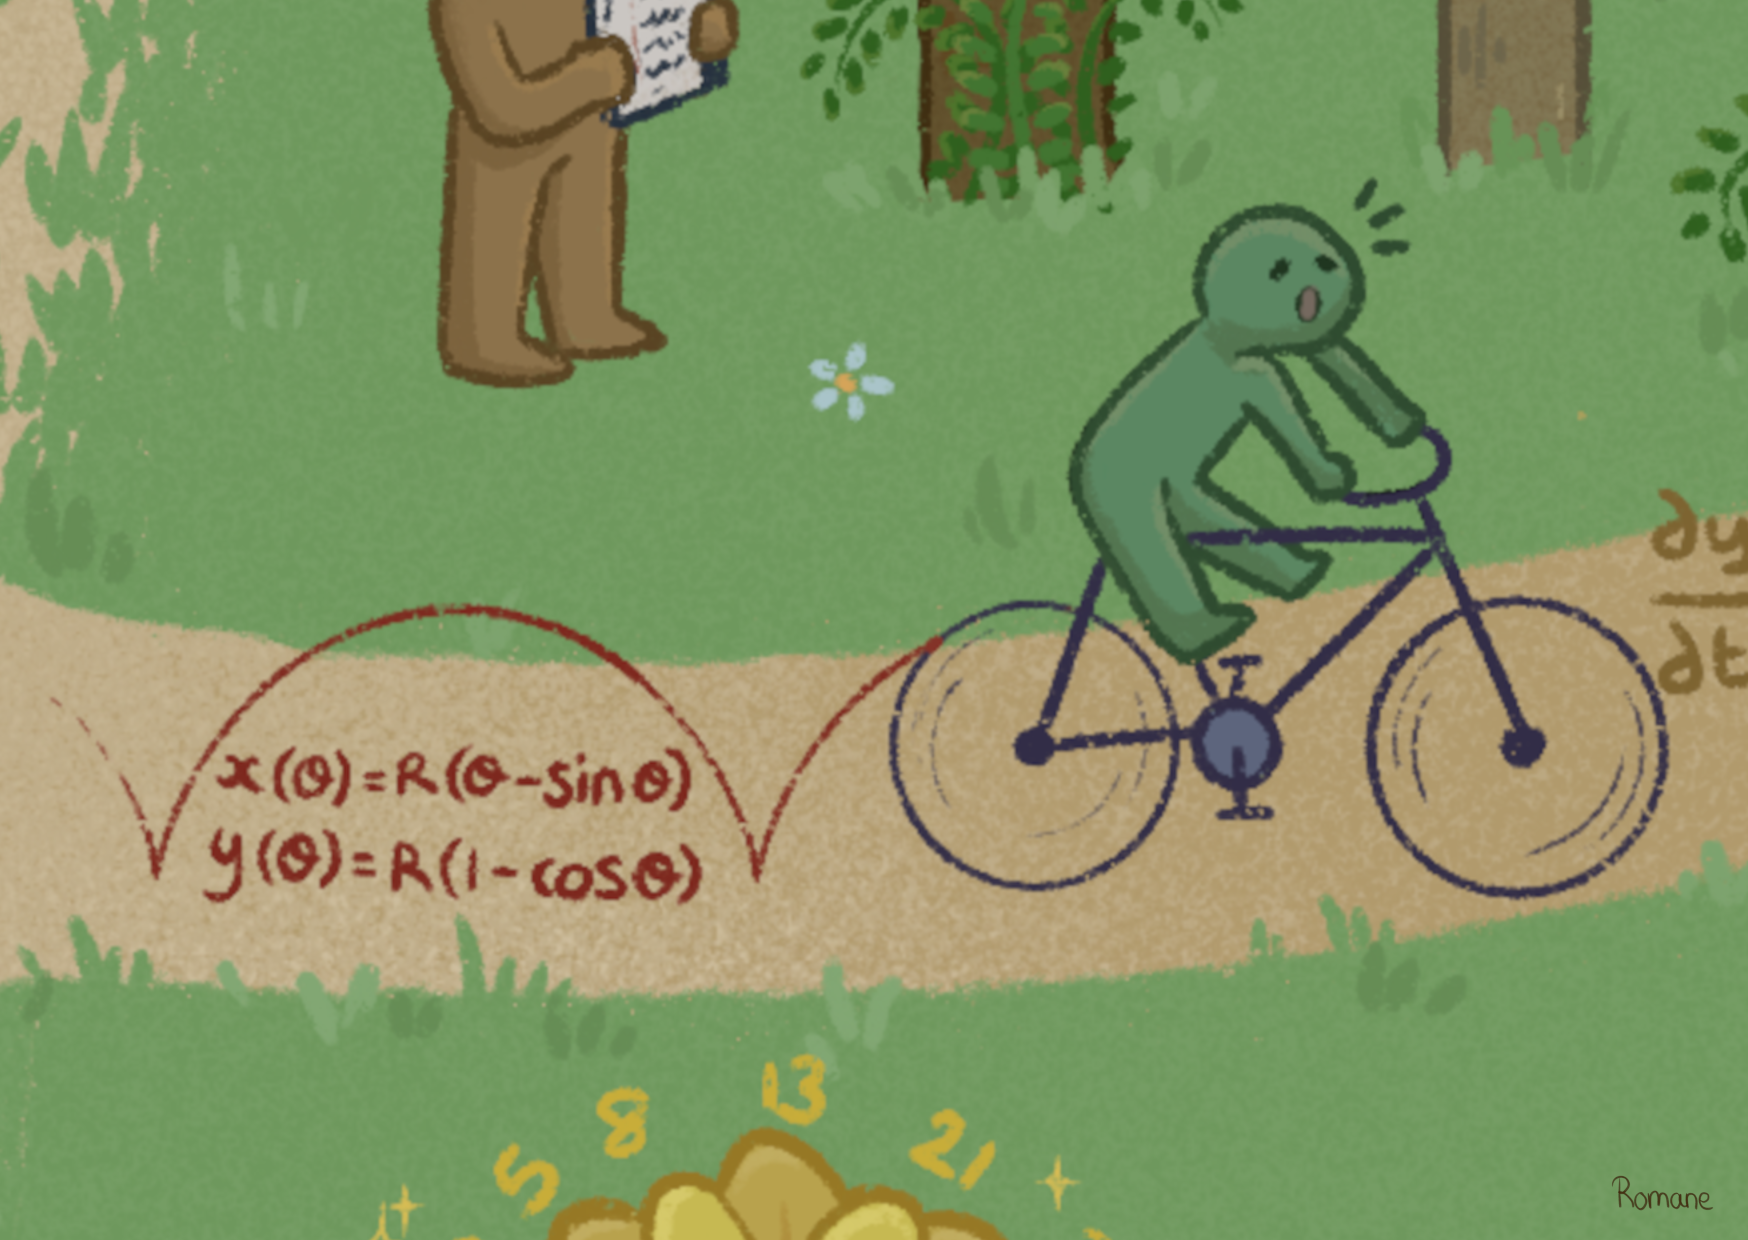
\includegraphics[height=0.5\textheight]{Cartes_postales/carte05-velo.png}\label{fig:c05}
    \caption{Carte postale: Velo}
\end{figure}

Le mouvement d'un point sur une roue de vélo est bien plus complexe qu'il n'y paraît. C'est la combinaison de deux mouvements simples, une translation et une rotation. Cela crée une courbe qu'on appelle une cycloïde, qui a des propriétés étonnantes.

\begin{figure}[h]
    \centering
    \includegraphics[height=0.1\textheight]{Images/cycloide.png}\label{fig:c05_cycloide}
    \caption{Illustration d'une cycloide inversée}
\end{figure}

Tout d'abord, en retournant cette courbe, c'est le chemin le plus rapide pour une bille de se déplacer d'un point A en hauteur à un point B plus bas. Puis, peut importe la position de départ de la bille sur cette courbe, la bille mettra toujours le même temps pour arriver tout en bas. Cette dernière propriété paraît très contre-intuitive, et pourtant ça marche super bien. L'étude de cette courbe a ouvert un champs entier en mathématiques appelé le calcul variationnel, sur lequel il y a beaucoup de recherches en cours. Voici comment on la définit:

\begin{equation*}
    \begin{cases} 
    x(\theta) = R(\theta - \sin \theta) \\
    y(\theta) = R(1 - \cos \theta) 
    \end{cases}
\end{equation*}
    \newpage
\section{Musique}

\begin{figure}[h]
    \centering
    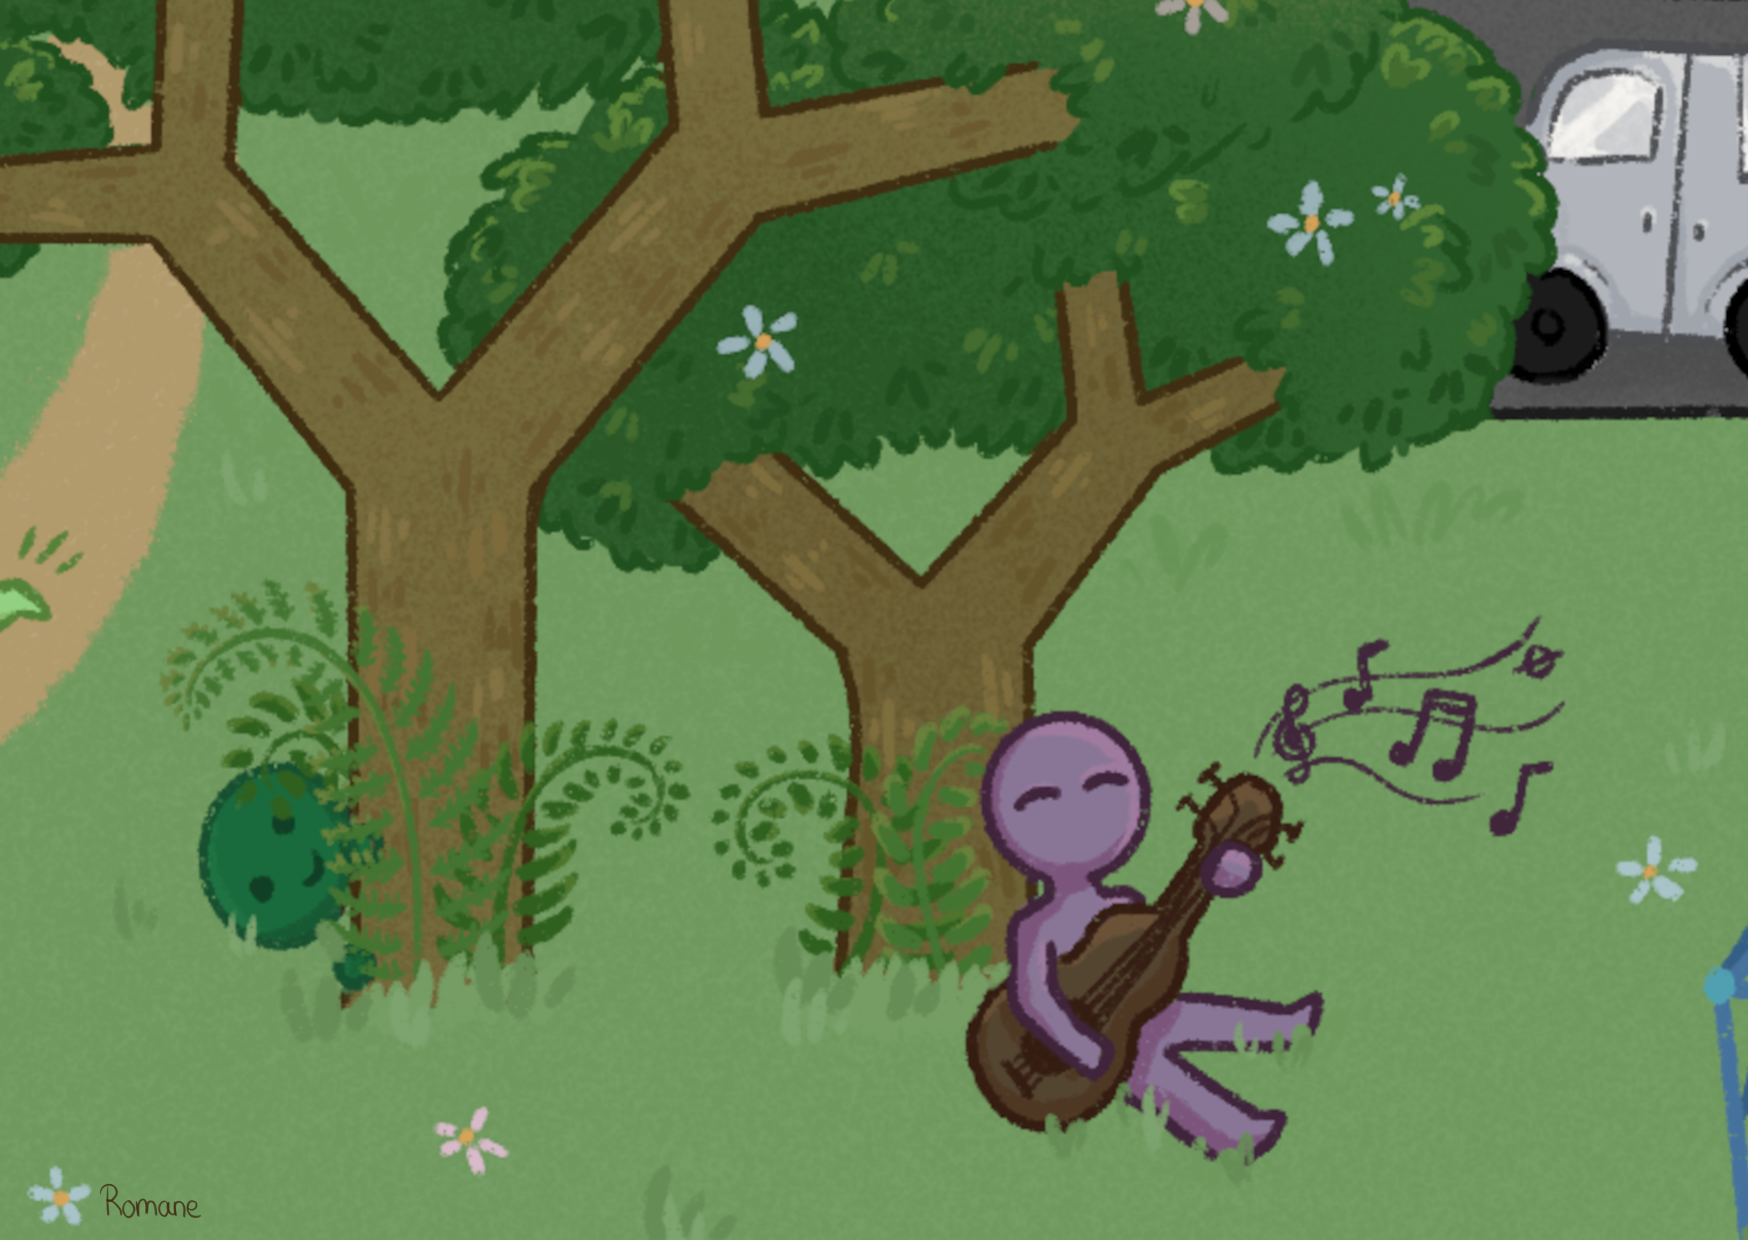
\includegraphics[height=0.5\textheight]{Cartes_postales/carte06-musique.png}\label{fig:c06}
    \caption{Carte postale: Musique}
\end{figure}

Sais-tu que la musique que nous écoutons repose sur un conflit mathématique insoluble? Une note de musique est une vibration de l'air, et deux notes sont harmonieuses si le rapport de leurs fréquences est une fraction simple: le rapport $2$ correspond à l'octave, tandis que le rapport $3/2$ définit la quinte. Pour construire une échelle musicale, une gamme, on cherche donc à utiliser ces deux intervalles. Cependant, en accumulant douze quintes successives, on obtient une valeur très proche mais différente de sept octaves cumulées: \[(3/2)^{12} \approx 129,746, \text{alors que } 2^7 = 128.\]

Cette infime différence, appelée le comma pythagoricien, empêche les cycles de notes de se refermer parfaitement, ce qui crée inévitablement des dissonances à l'oreille. En pratique, comme il est impossible d'obtenir une gamme où toutes les quintes et toutes les octaves sont parfaitement pures, les musiciens ont dû faire un compromis: la "gamme tempérée". En multipliant la fréquence de chaque note par un coefficient fixe de $2^{1/12}$, on répartit équitablement cette dissonance sur les douze notes de la gamme. En couplant cette théorie mathématique à notre système occidental, on accepte que les notes ne sonnent jamais de manière absolument pure, mais on réussit à éviter tout accord trop faux, permettant aux instruments de jouer harmonieusement dans toutes les tonalités.
    \newpage
\section{Montagne}

\begin{figure}[h]
    \centering
    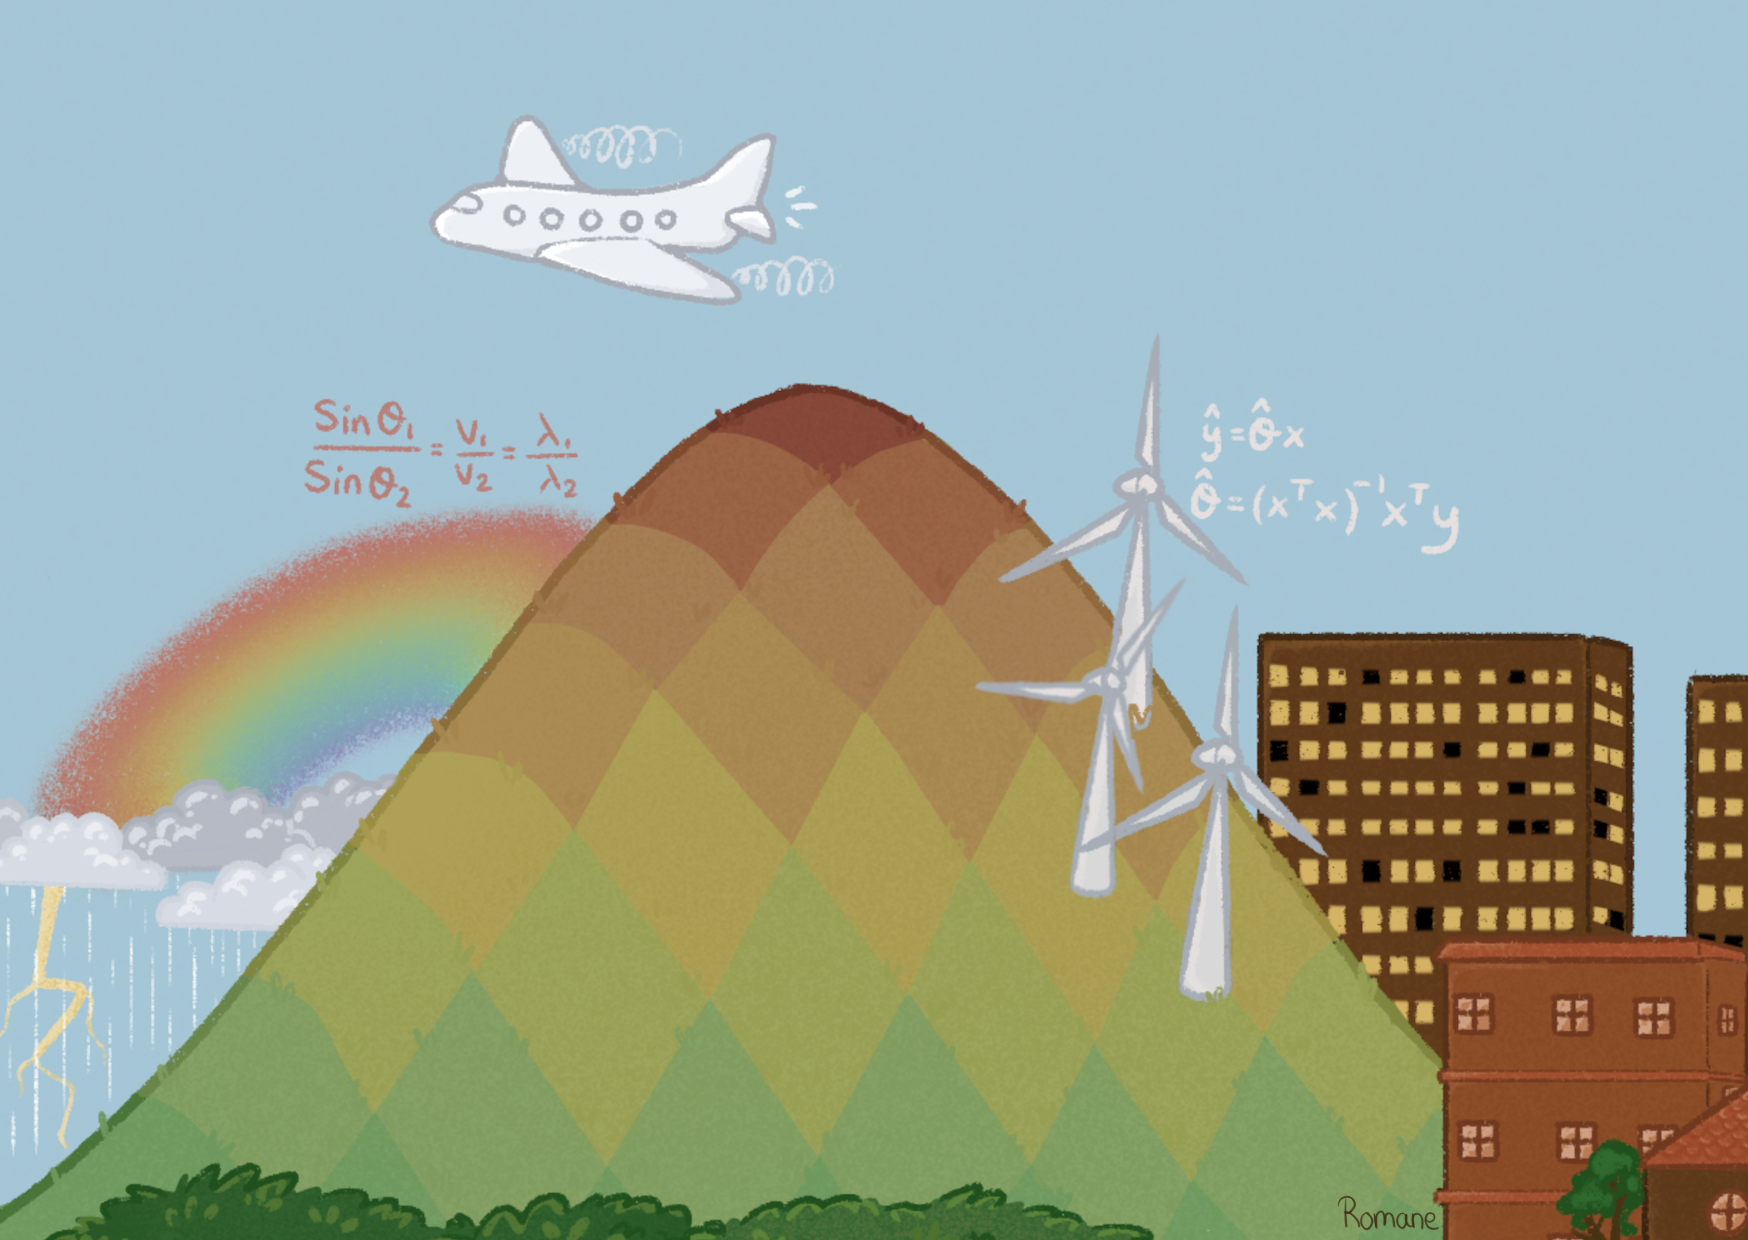
\includegraphics[height=0.5\textheight]{Cartes_postales/carte07-montagne.png}\label{fig:c07}
    \caption{Carte postale: Montagne}
\end{figure}

Sais-tu qu'on a des objets mathématiques avec des dimensions non entières? En géométrie classique, on étudie souvent des objets comme des segments, carrés, sphères ou d'autres formes simples, avec des dimensions entières, comme 1, 2 ou 3. La dimension permet de donner des précisions sur notre objet comme son périmètre et son aire. Cependant, il y a beaucoup de formes plus complexe où cette approche ne marche pas. Voici par exemple une fractale appelé la fractale de Sierpinski. On part d'un triangle équilatéral, qu'on découpe en 4 triangles équilatéraux et on retire le triangle central. Puis on recommence dans chaque triangle, indéfiniment. Avec une approche classique, on obtient une surface infini et une aire nulle en dimension 2. Donc pas très utile pour comprendre ce qui se passe.

\begin{figure}[h]
    \centering
    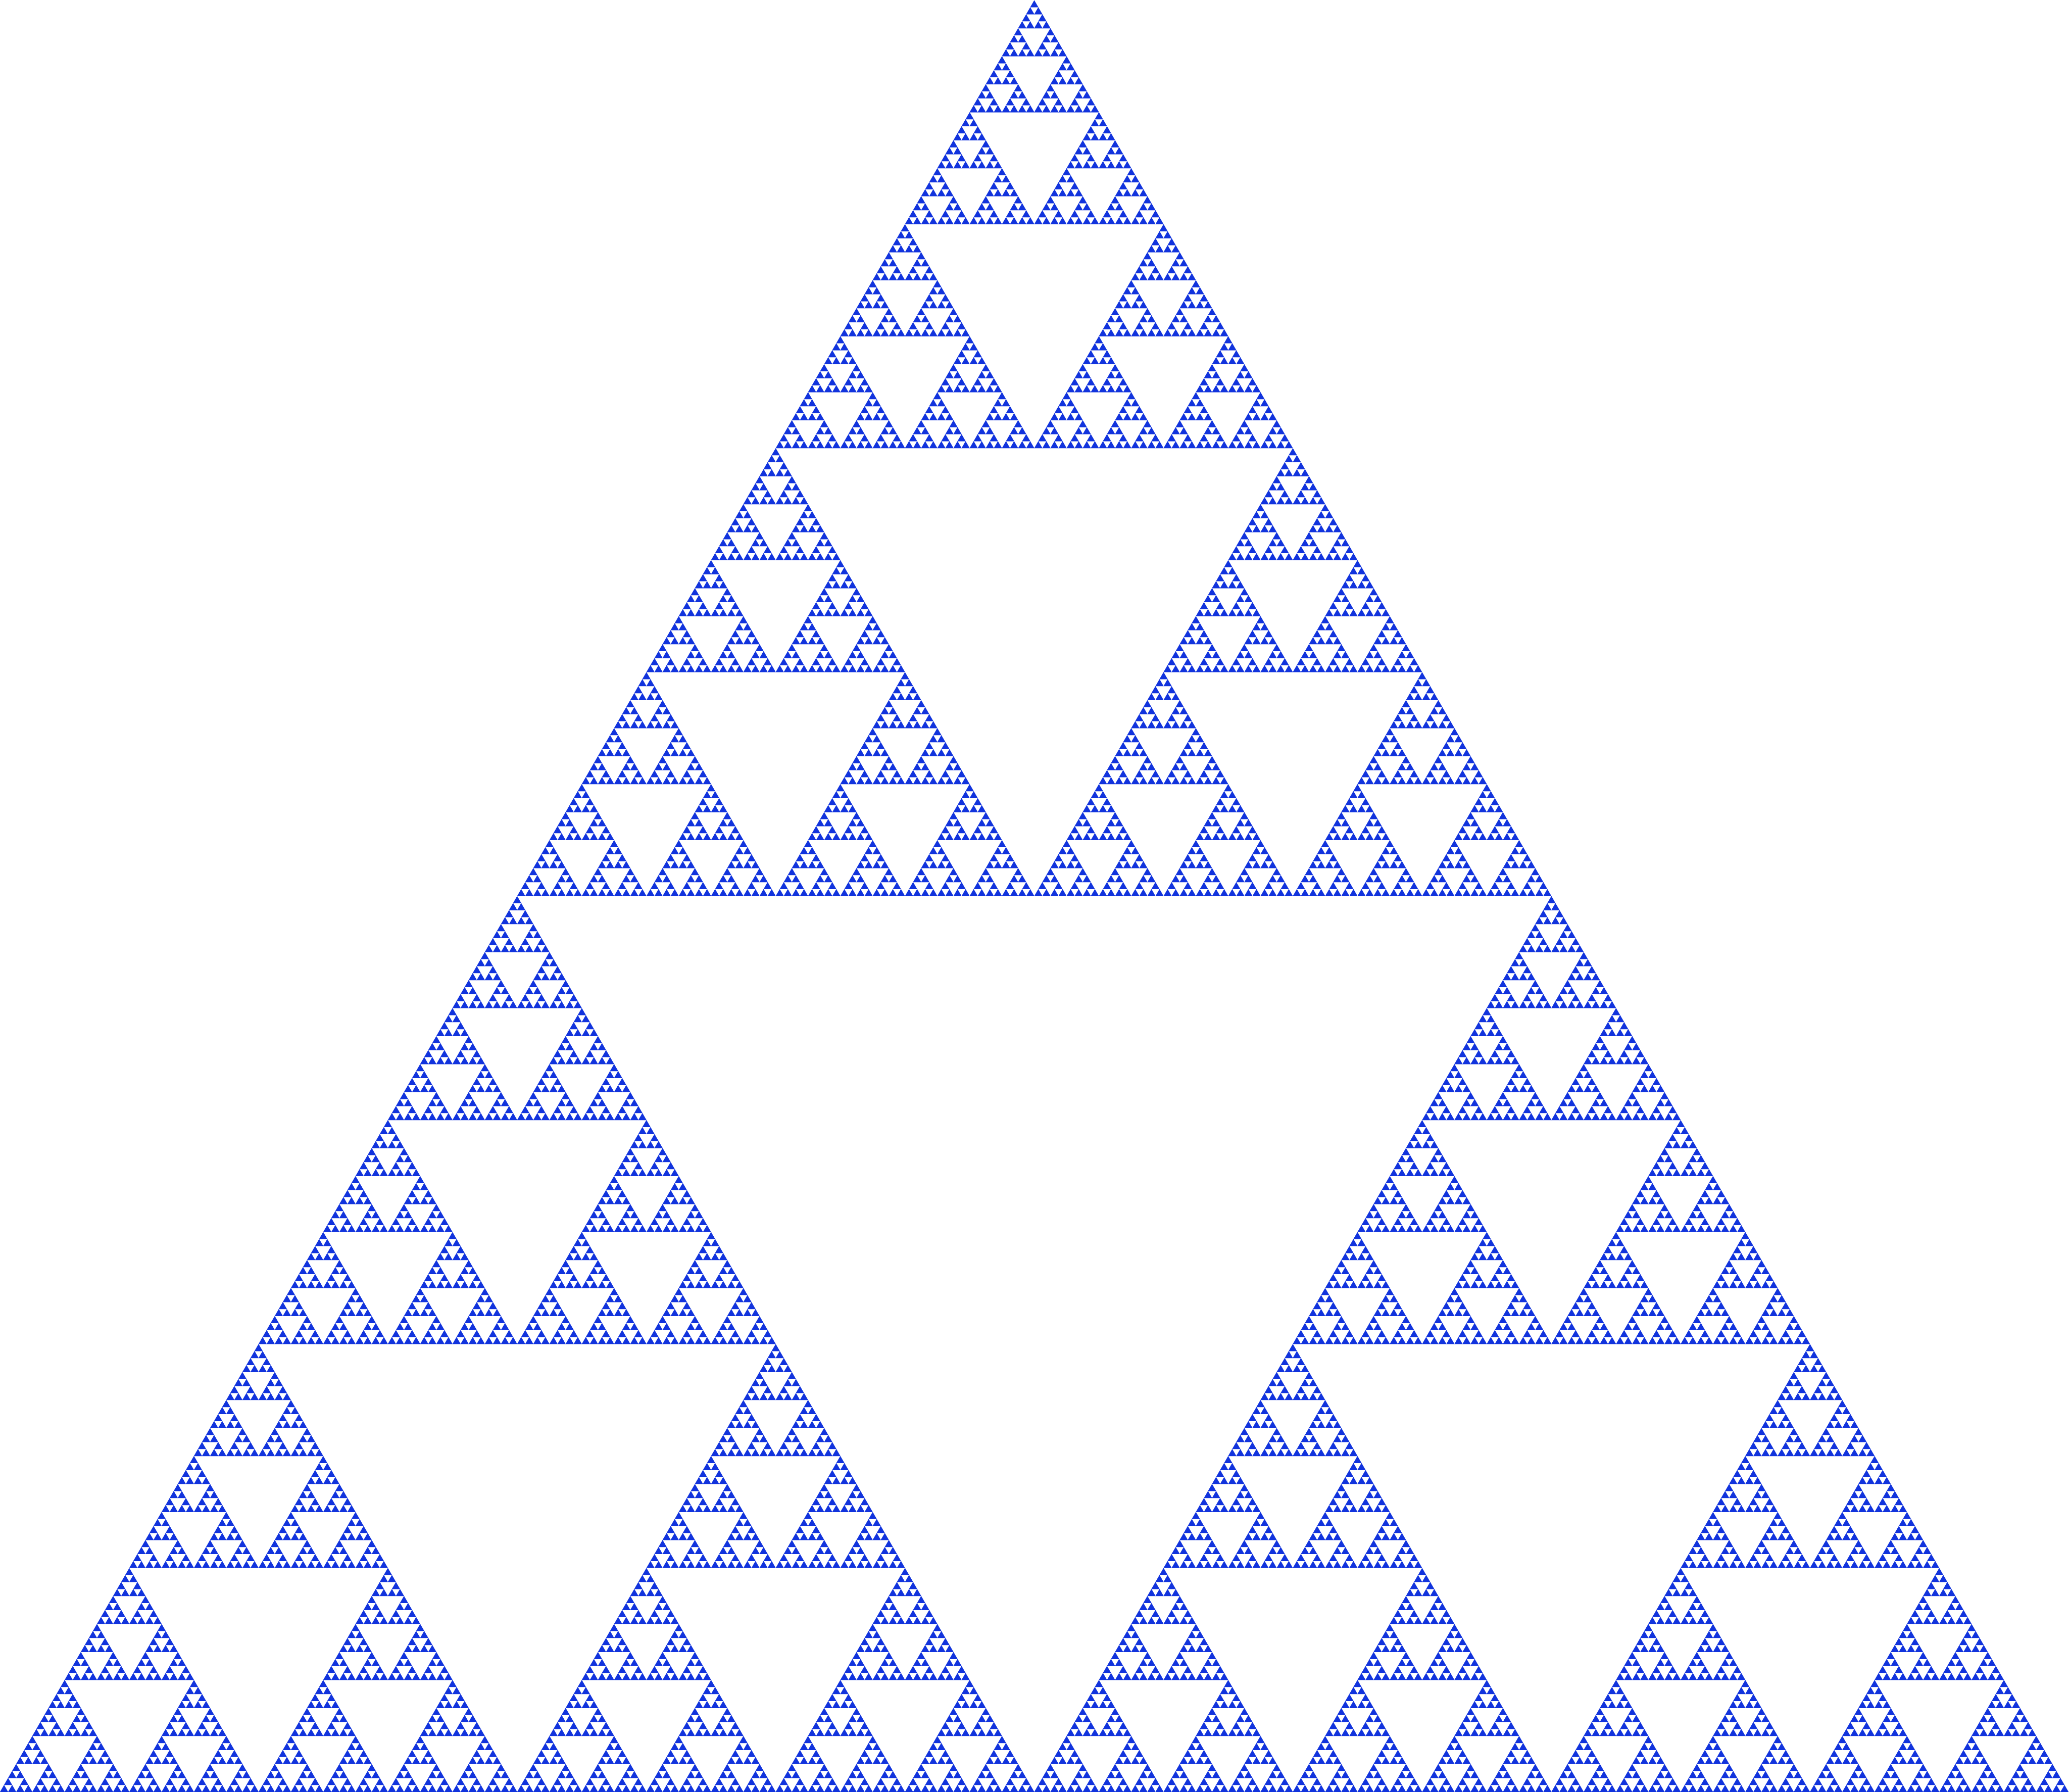
\includegraphics[height=0.1\textheight]{Images/sierpinski.png}\label{fig:c07_sierpinski}
    \caption{Le triangle de Sierpinski}
\end{figure}


En géométrie fractale, on étend cette notion de dimension, ce qui va nous donner une idée de la rugosité de notre objet. Si notre objet est très similaire à un segment, sa dimension sera proche de 1, et si il est chaotique comme la côte d'Angleterre, il aura une dimension plus grande comme 1,2. Ici, la dimension de cette fractale est d'environ 1,585. Une mer calme a une dimension fractale autour de 2,05 à 2,1 par exemple alors que la chaîne de montagnes en Himalaya, aura une dimension fractale plus proche de 2,4 ou 2,6. La dimension fractale est très importante car elle peut être utilisé dès qu'il y a des différences de comportements dans ce qu'on étudie. Elle est utilisé dans de nombreux domaines, comme en imagerie médicale pour détecter des tumeurs par exemple (car des cellules saines sont très organisées alors que des cellules cancéreuses sont plus chaotiques, et donc leur dimensions fractales sont différentes).
    \newpage
\section{Maison}

\begin{figure}[h]
    \centering
    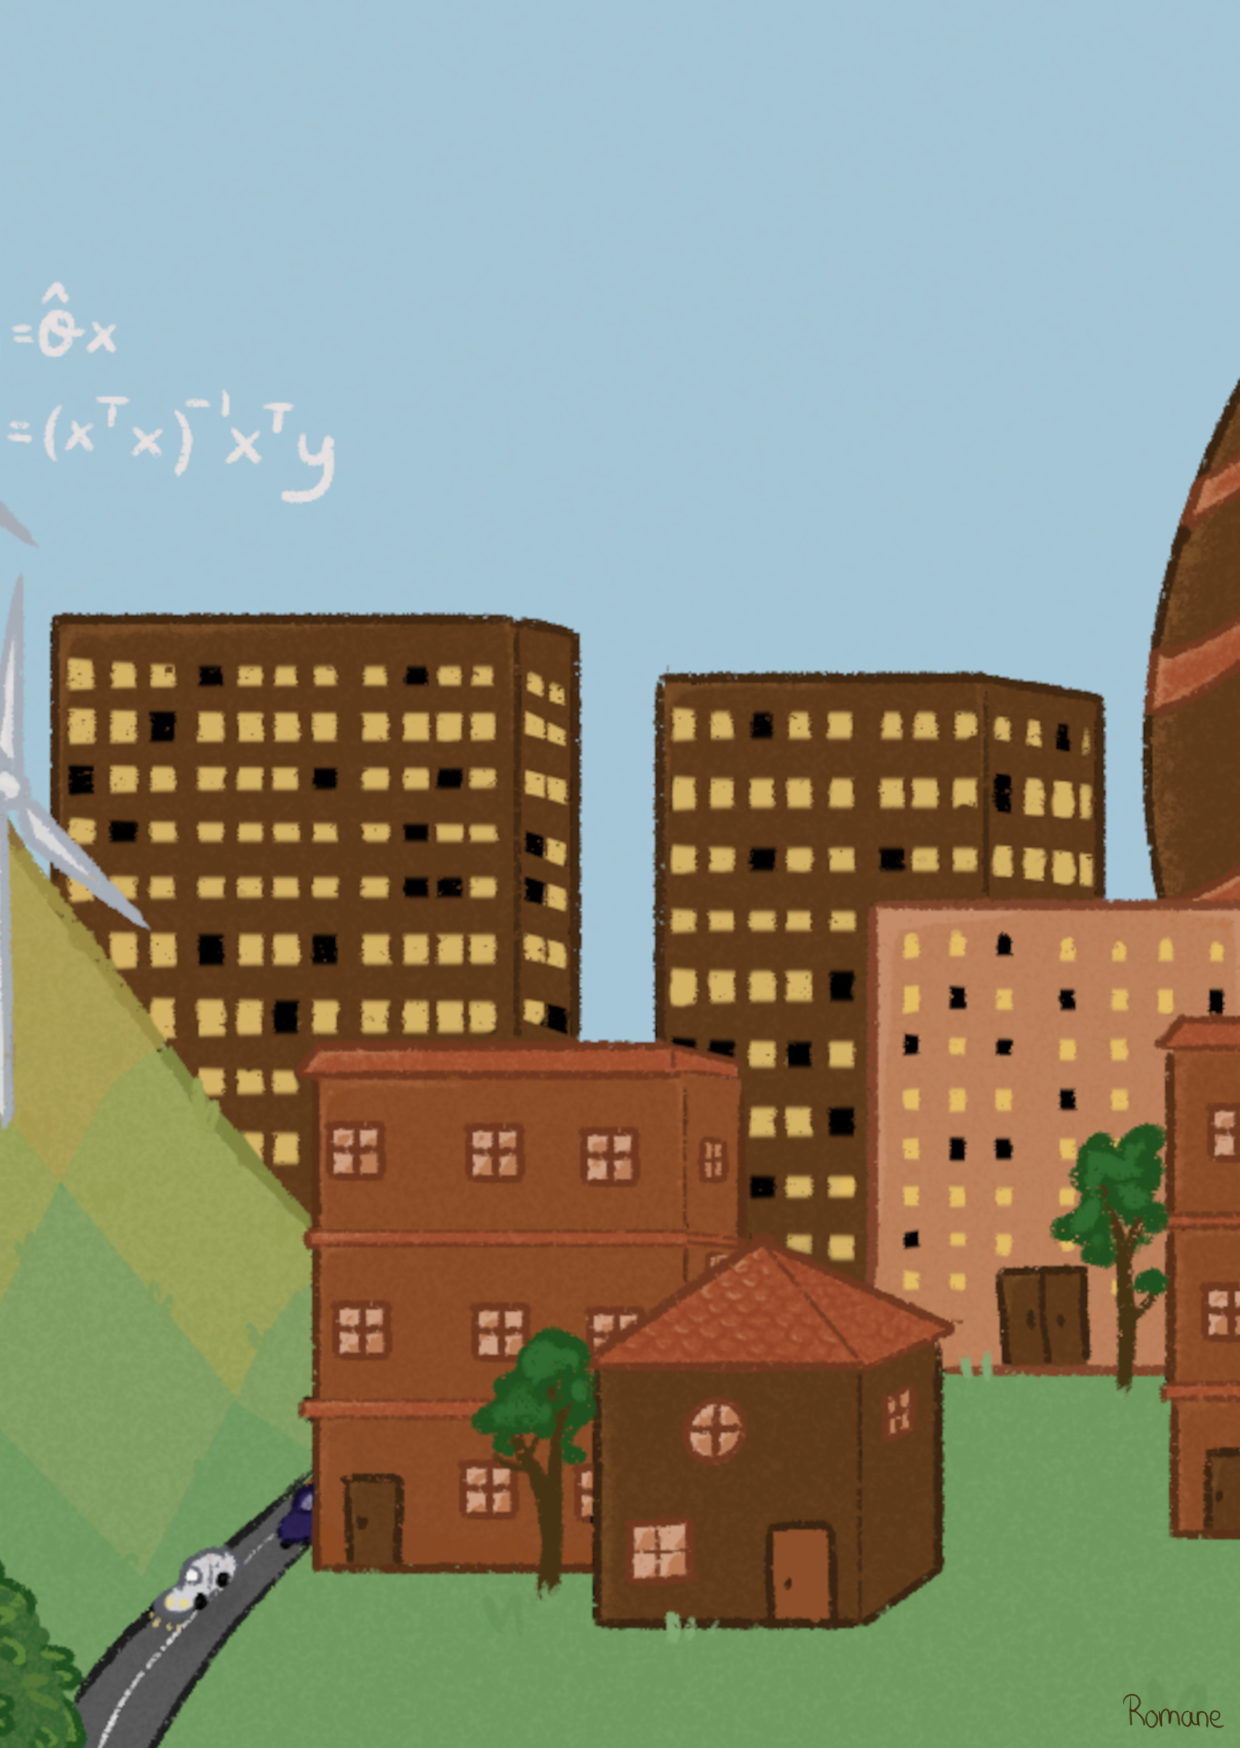
\includegraphics[height=0.5\textheight]{Cartes_postales/carte08-maison.png} 
    \label{fig:mon_image}
    \caption{Carte postale: Maison}
\end{figure}



    \newpage
\section{Proie}

\begin{figure}[h]
    \centering
    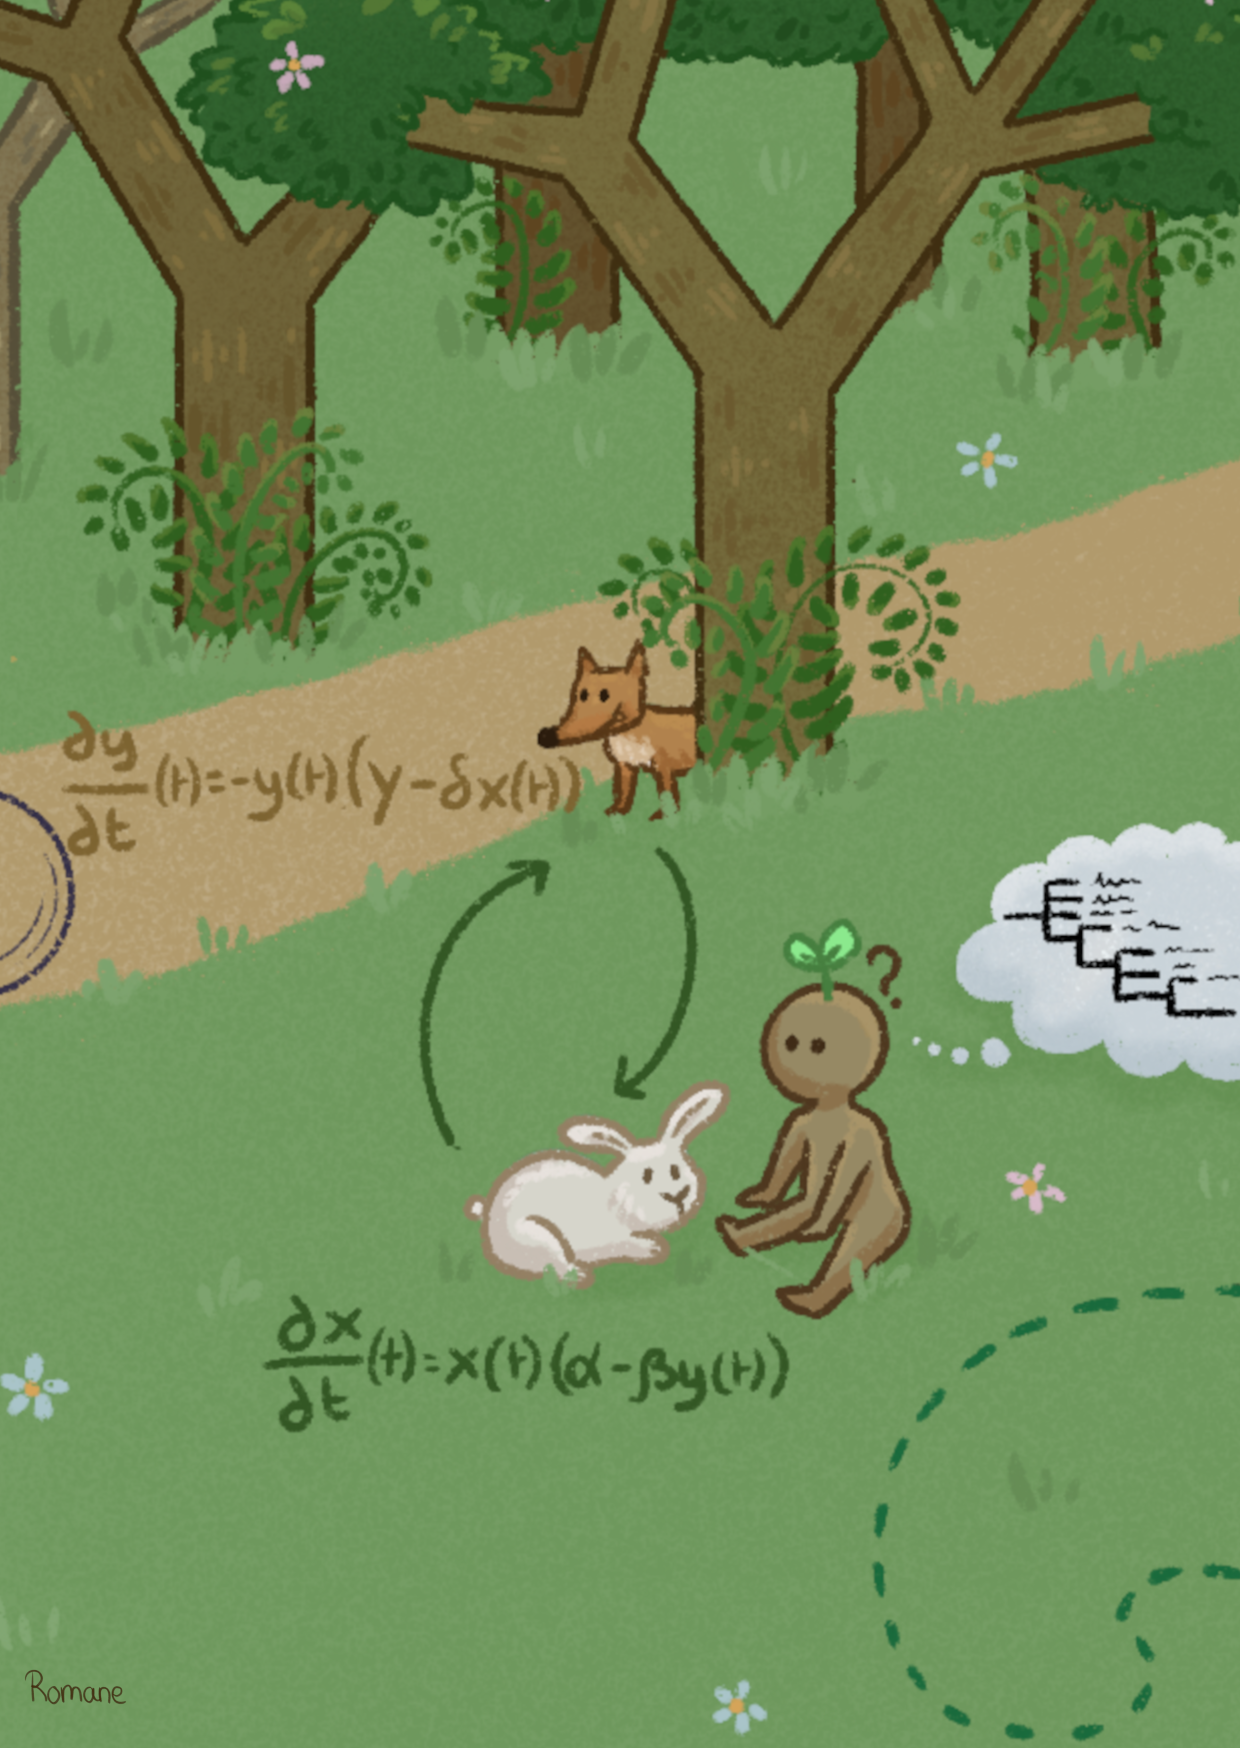
\includegraphics[height=0.5\textheight]{Cartes_postales/carte09-proie.png}\label{fig:c09}
    \caption{Carte postale: Proie}
\end{figure}

Sais-tu qu'on peut modéliser l'évolution des populations de lapins et renards? Lorsqu'il y a beaucoup de lapins, les renards trouvent facilement de la nourriture et leur population augmente. Mais plus il y a de renards, plus les lapins sont mangés et donc le nombre de lapins finit par diminuer. Les renards ont alors plus de difficultés à se nourrir et leur population baisse à son tour. Les lapins, ayant moins de prédateurs, peuvent ensuite se multiplier à nouveau, et le cycle recommence. Les équations ci-dessous permettent de formaliser ce cycle:

\[
\frac{dR(t)}{dt}=-R(t)(a-bL(t))
\]
\newline
\[
\frac{dL(t)}{dt}=L(t)(c-dR(t))
\]

Ce cycle très célèbre est appelé le modèle proie-prédateur et il est très utile pour étudier des populations. Lorsqu'on étudie des populations, on va souvent rencontrer un équilibre stable, le nombre de lapins et renards va se stabiliser autour d'une certaine valeure. Plus l'environnement et les conditions de survie sont stable, plus l'équilibre est durable. Et si les paramètres changent brutalement, comme avec l'arrivée d'une maladie, cet équilibre va se rompre et on va atteindre un nouvel équilibre stable, après une période de grands changements.
    \newpage

\section{marche aléatoire}

\begin{figure}[h]
    \centering
    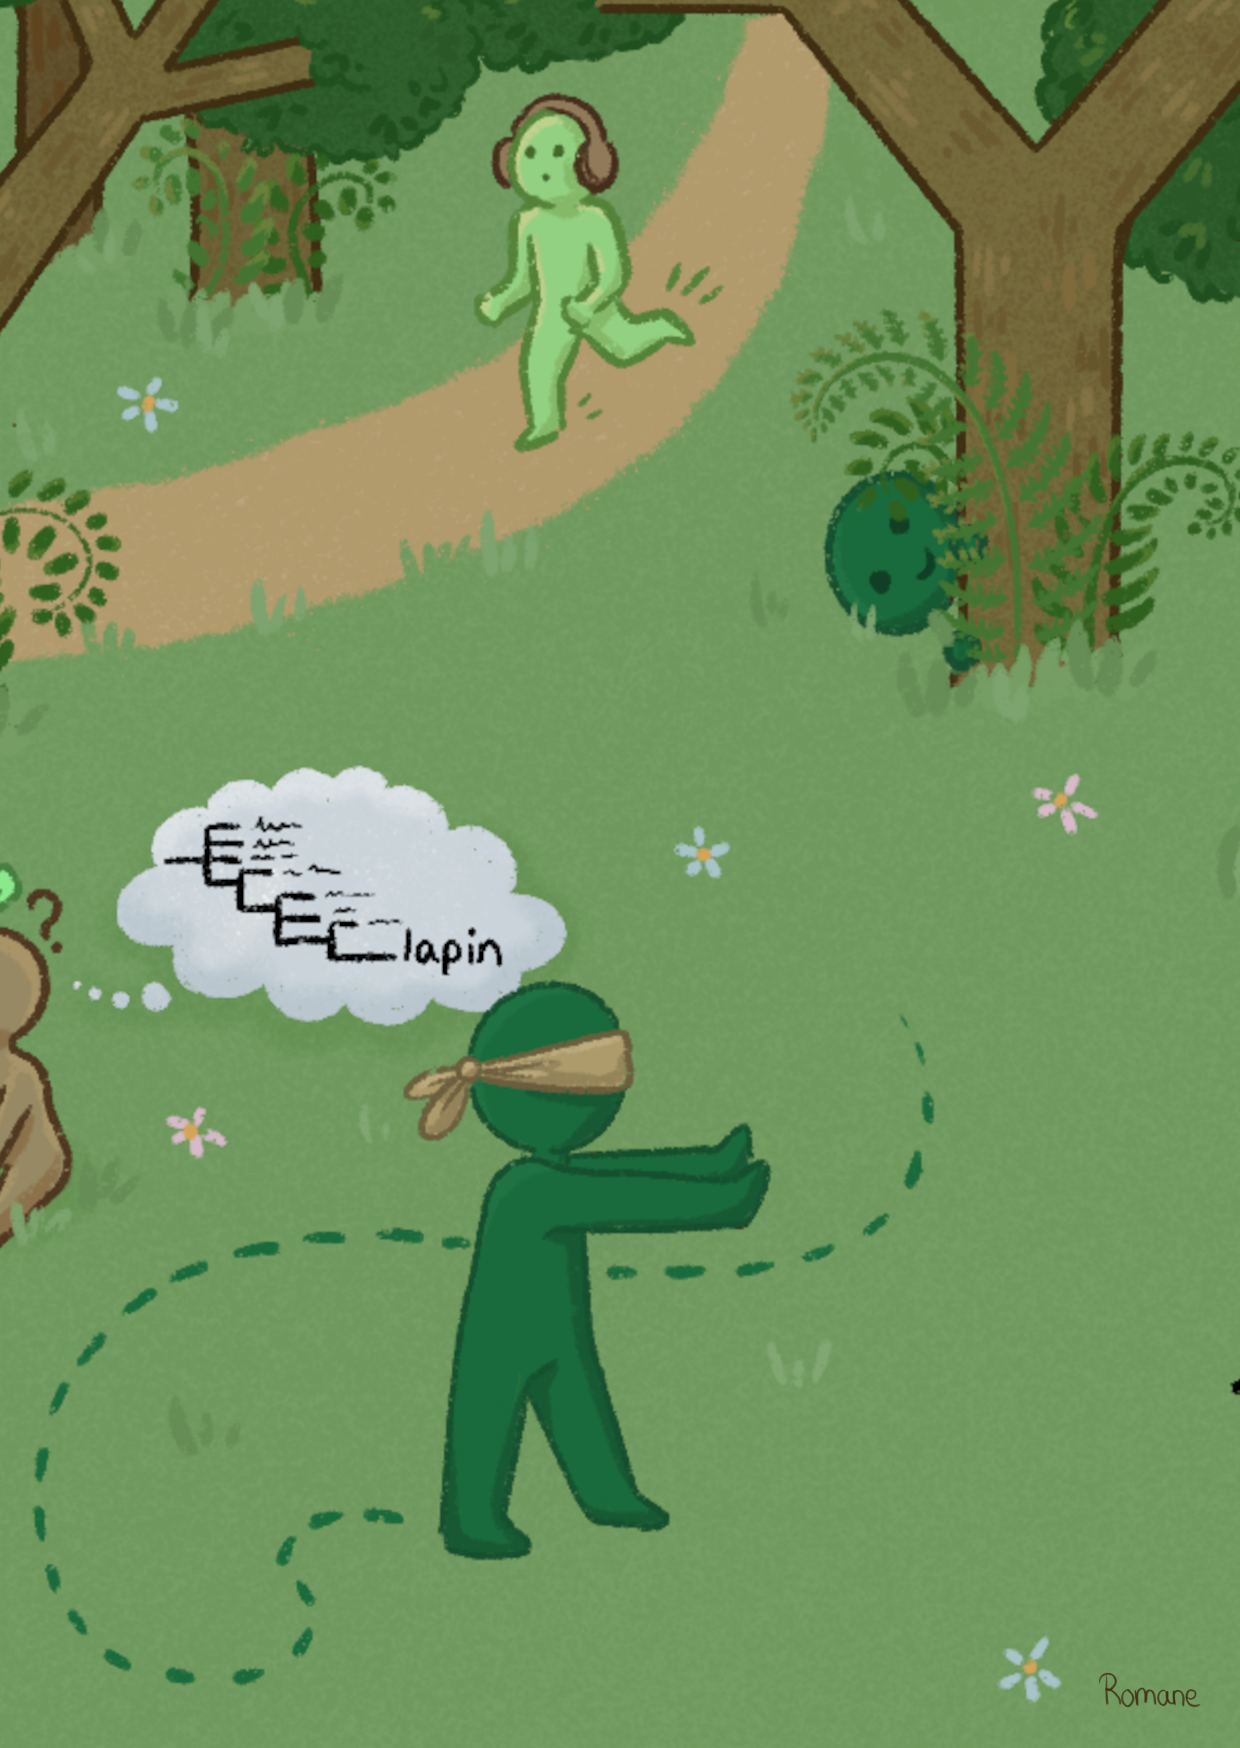
\includegraphics[height=0.5\textheight]{Cartes_postales/carte10-marche.png}\label{fig:c10}
    \caption{Carte postale: marche}
\end{figure}

Imaginons que tu te retrouves au milieu des rues de Manhattan, à New York, et tu commences à marcher. A chaque intersection, tu choisis aléatoirement la direction que tu prends. Si tu continues ce processus indéfiniment, tu finiras toujours par revenir à ton point de départ. Et ce, même s'il y avait une infinité de rues. Les probabilités permettent de trouver de l'ordre dans le chaos en établissant des lois universelles sur des comportements imprévisibles.
\medskip

C'est un concept très utile pour modéliser le hasard au quotidien, comme la trajectoire des molécules d'un parfum qui se diffuse dans une pièce ou les fluctuations de la bourse. En pratique, le monde réel complexifie les calculs (interactions physiques, crises financières), ce qui pousse les mathématiciens à chercher des modèles toujours plus précis. En couplant ces théories à des données de qualité, on réussit à prédire l'imprévisible grâce à des intervalles de confiance. \\



    \newpage
\section{Ruche}

\begin{figure}[h]
    \centering
    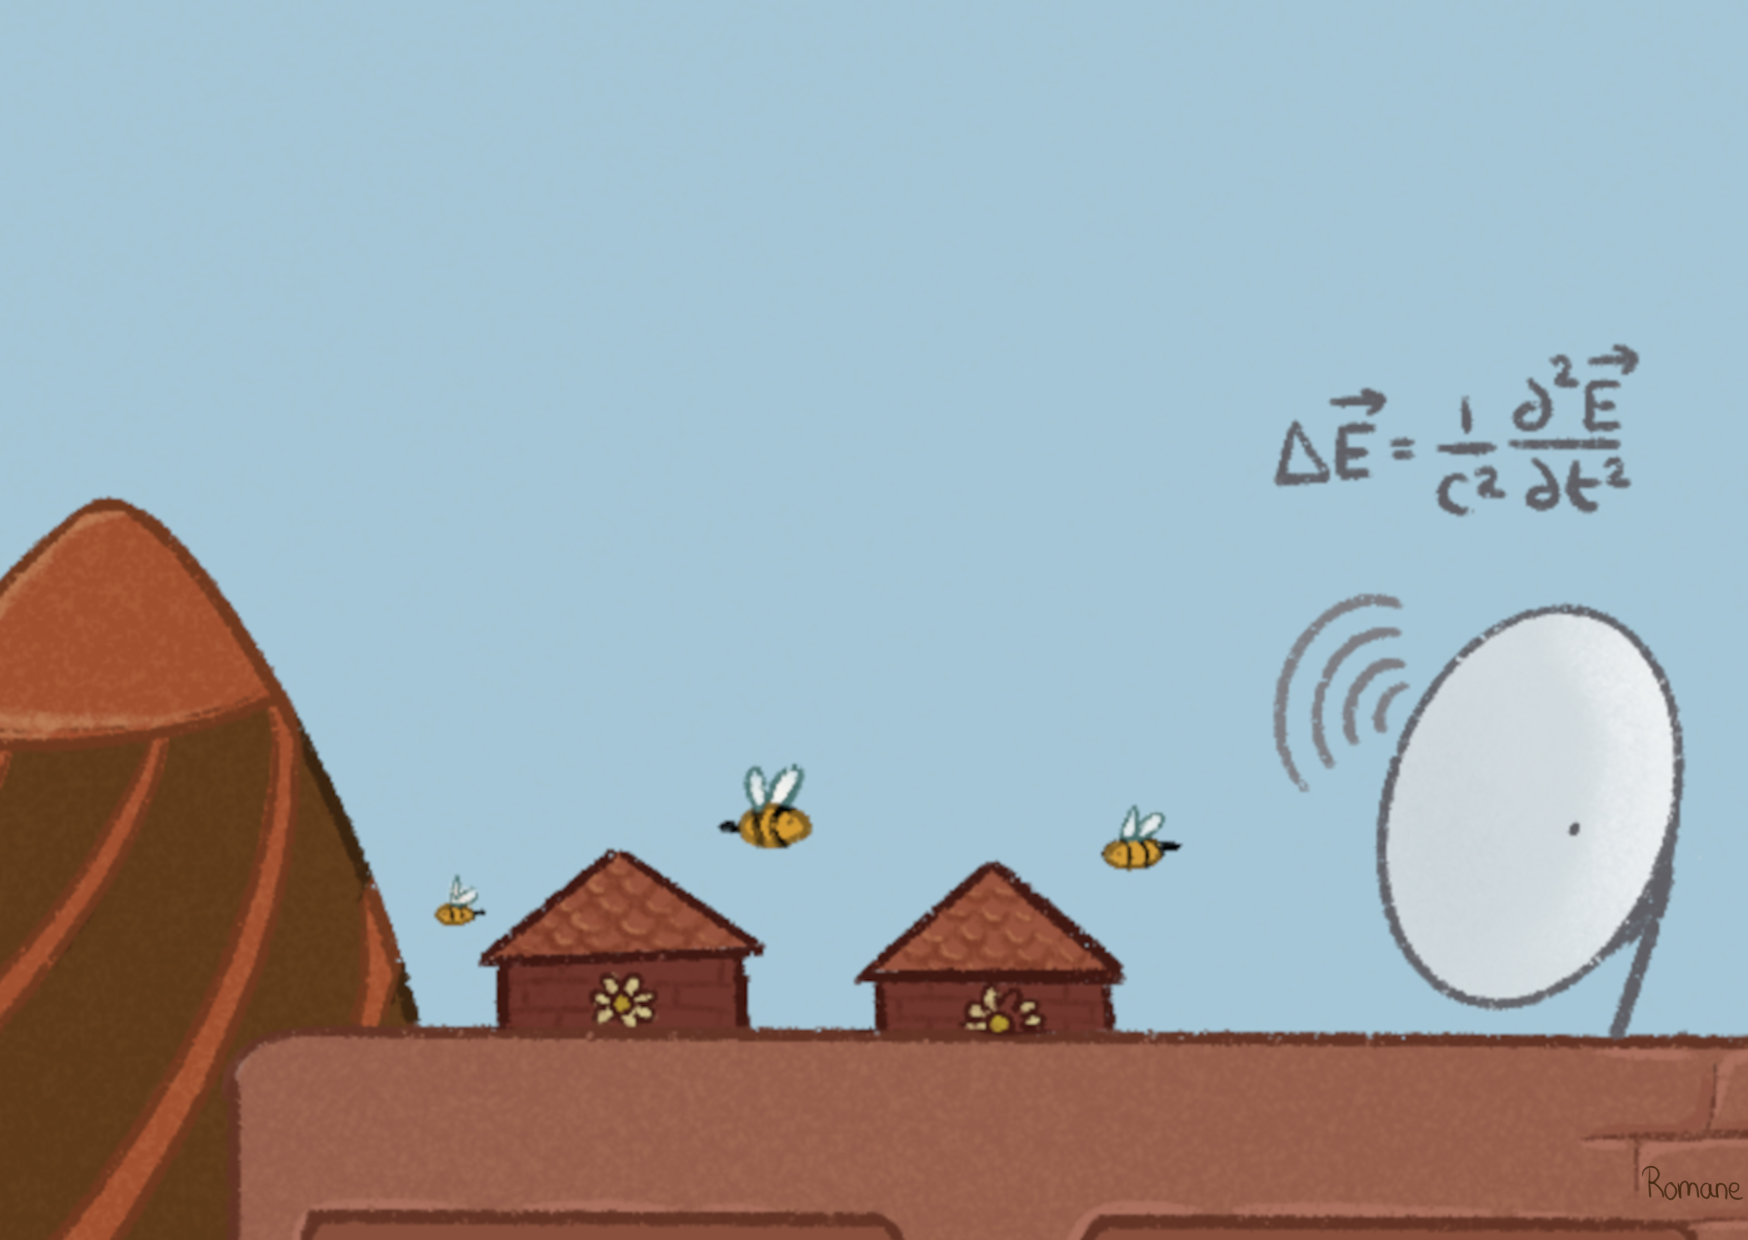
\includegraphics[height=0.5\textheight]{Cartes_postales/carte11-ruche.png} 
    \label{fig:mon_image}
    \caption{Carte postale: Ruche}
\end{figure}


    \newpage
\section{Phare}

\begin{figure}[h]
    \centering
    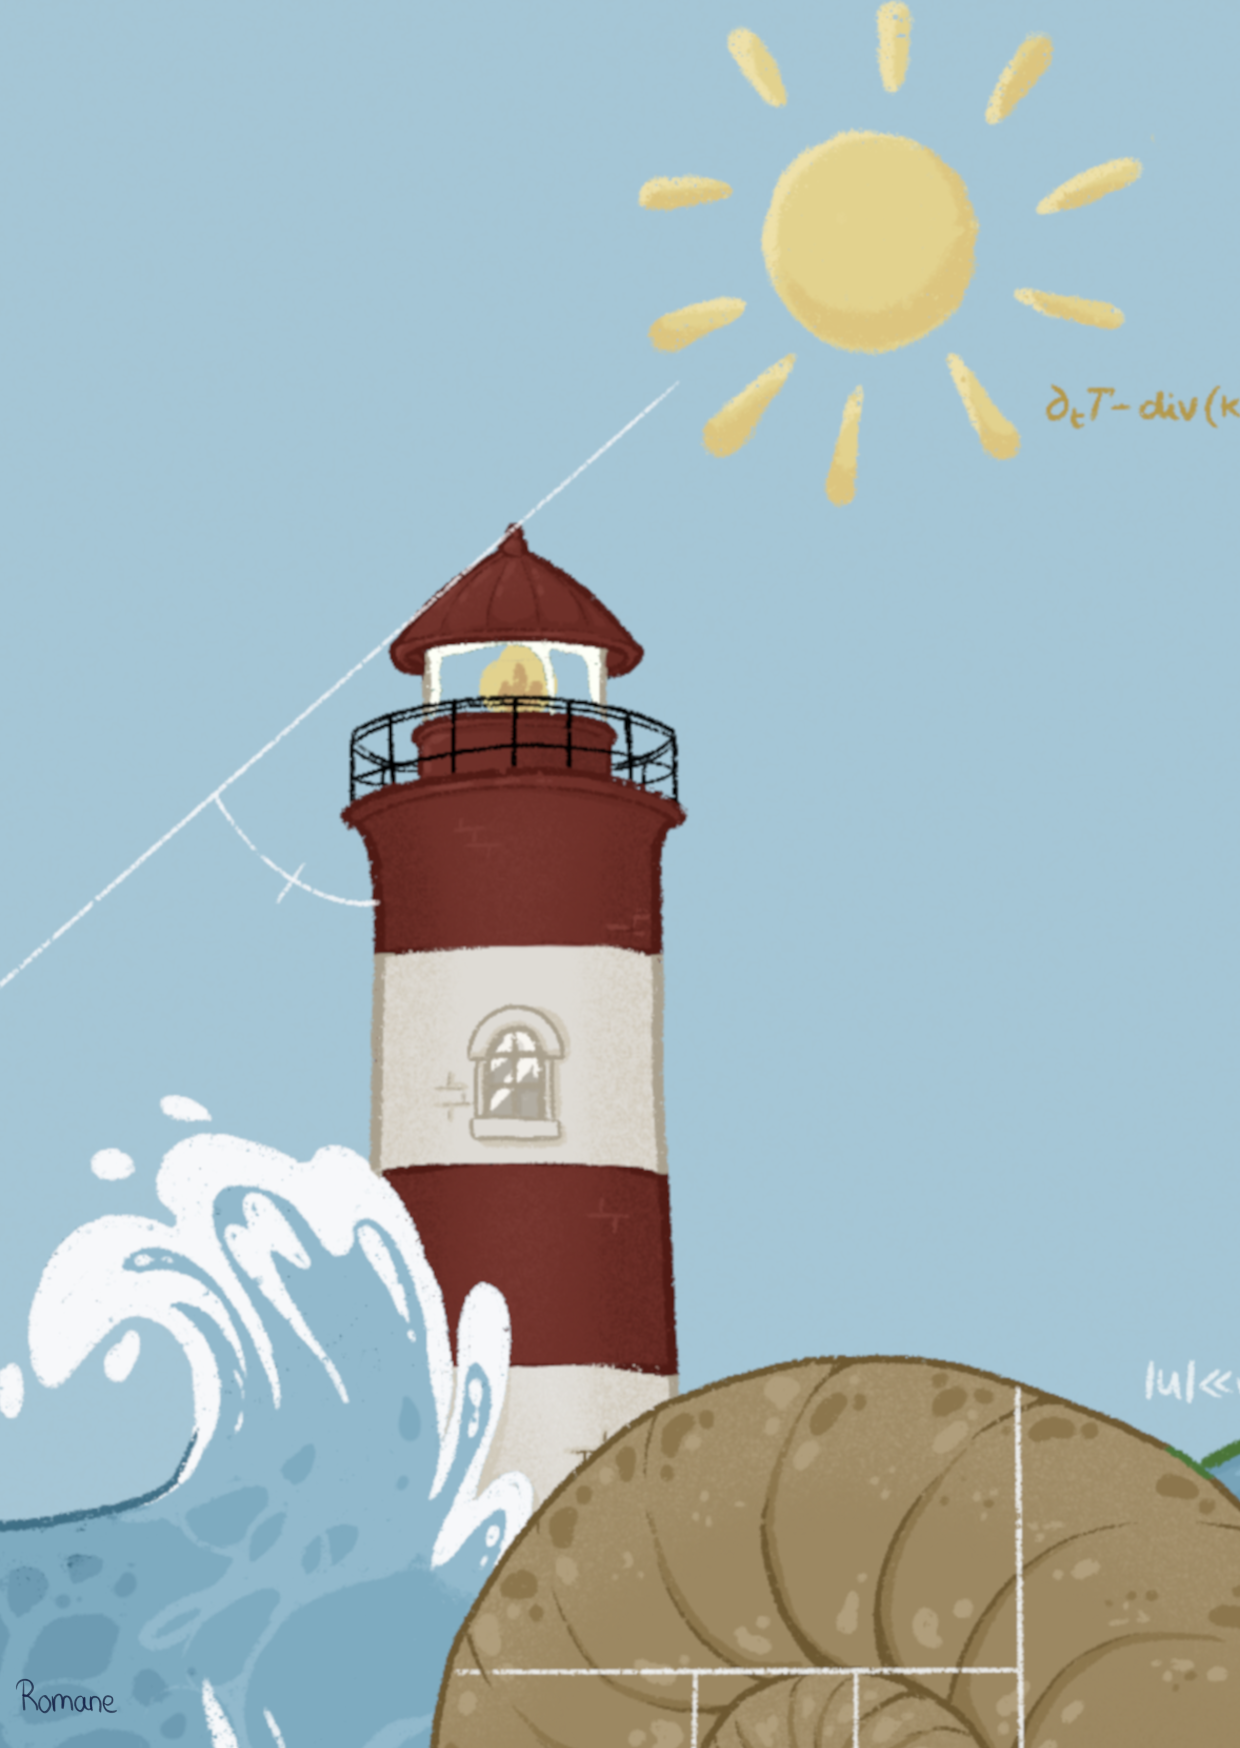
\includegraphics[height=0.5\textheight]{Cartes_postales/carte12-phare.png}\label{fig:c12}
    \caption{Carte postale: Phare}
\end{figure}


Sais-tu qu'on peut calculer la température à l'intérieur du Soleil? Au coeur du soleil, il y a des réactions nucléaires qui se produisent en permanence, libérant une immense quantité d'énergie. Cette énergie se propage ensuite vers la surface sous forme de chaleur et de rayonnement lumineux. En physique, nous sommes capable d'étudier et déterminer ces grandeurs à travers l'équation de la chaleur, où l'évolution de la température dépend de la quantité d'énergie produite et du milieu dans lequel la chaleur se propage.

\[
\partial_t T - \operatorname{div}(K \nabla T) = S
\]

On peut déterminer ces grandeurs en résolvant cette équation avec un ordinateur et en comparant nos résultats avec des observations réelles de la température à différents endroits à la surface du Soleil. Cela nous permet de faire des prédictions sur l'évolution de la température du Soleil, mais aussi de mieux comprendre comment le Soleil fonctionne et comment on peut s'y adapter.
    \newpage
\section{Lunette}

\begin{figure}[h]
    \centering
    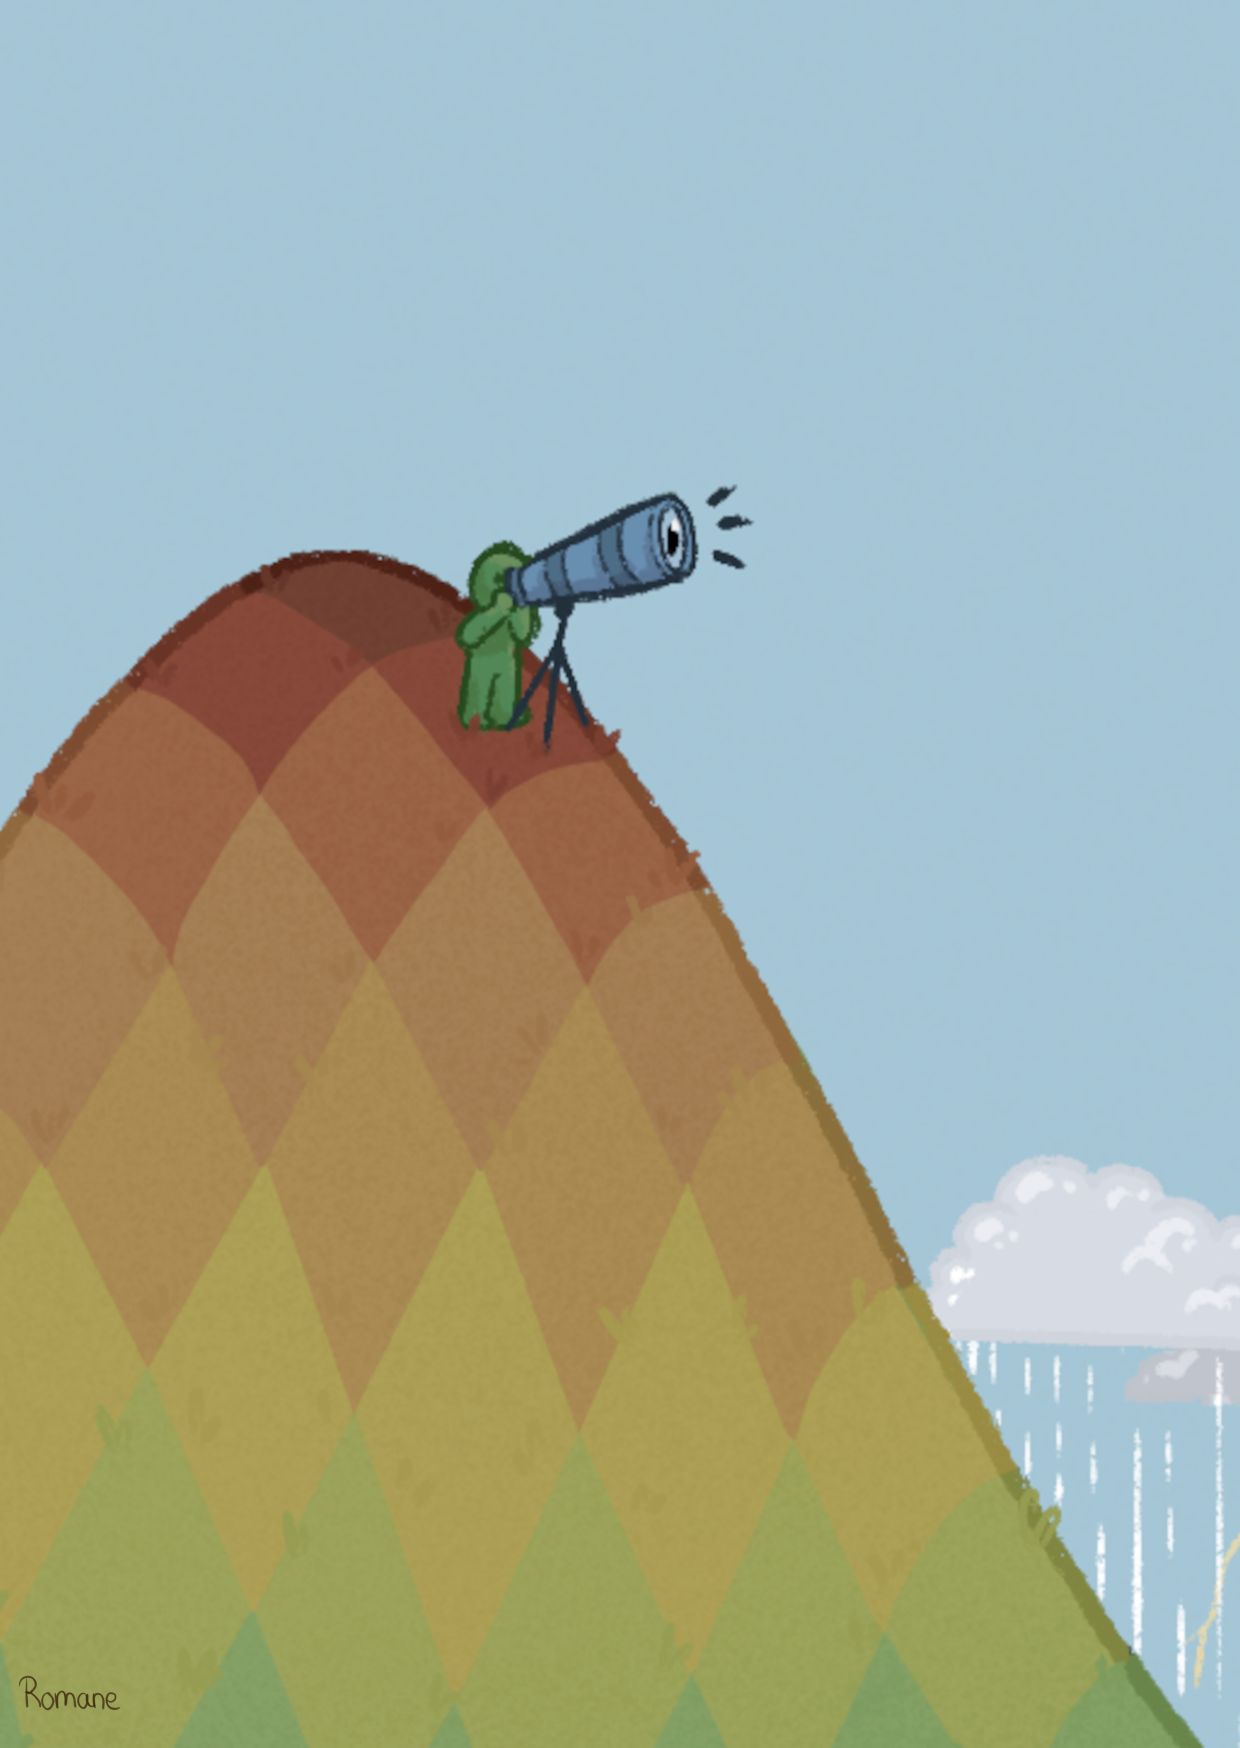
\includegraphics[height=0.5\textheight]{Cartes_postales/carte13-lunette.png} 
    \label{fig:mon_image}
    \caption{Carte postale: Lunette}
\end{figure}


    \newpage
\section{Arbres}

\begin{figure}[h]
    \centering
    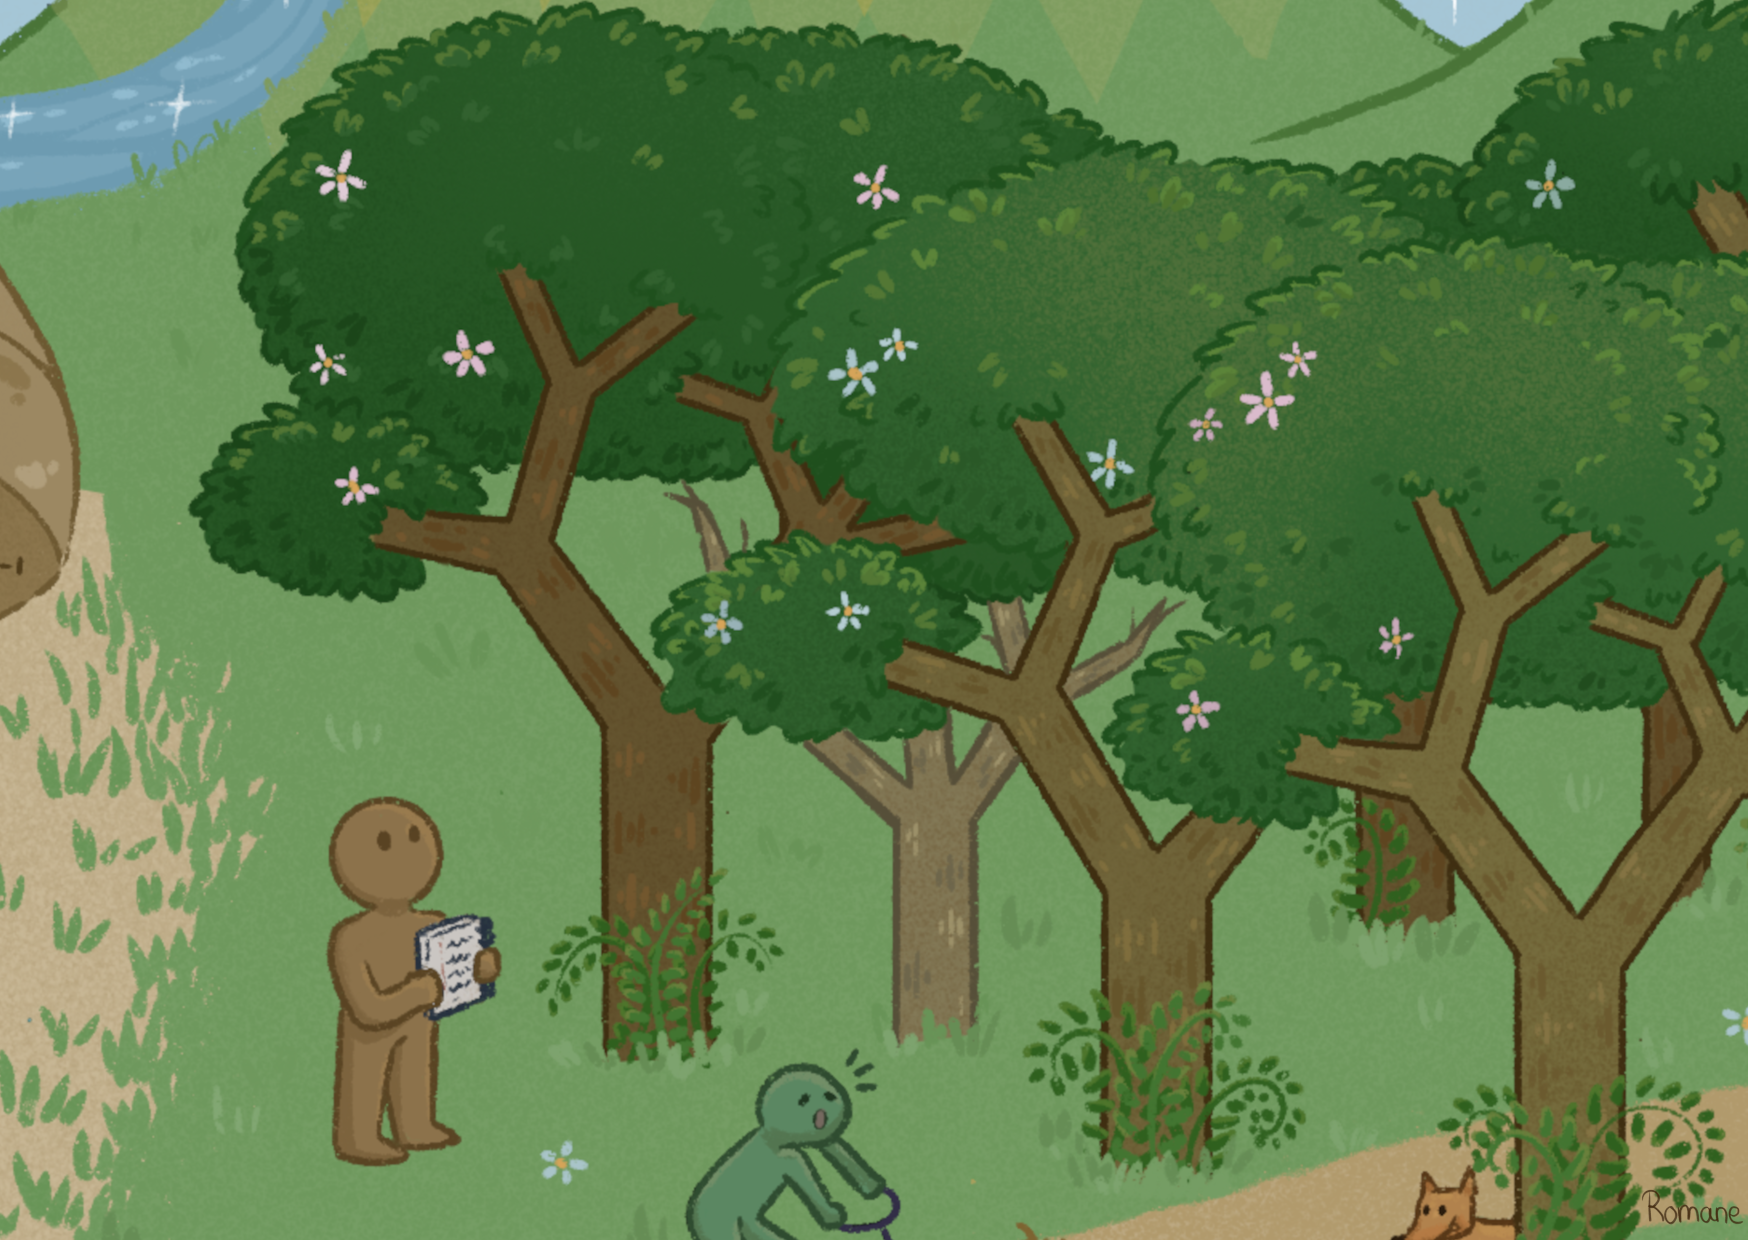
\includegraphics[height=0.5\textheight]{Cartes_postales/carte14-arbres.png} 
    \label{fig:mon_image}
    \caption{Carte postale: Arbres}
\end{figure}


    \newpage
\section{Bouee}

\begin{figure}[h]
    \centering
    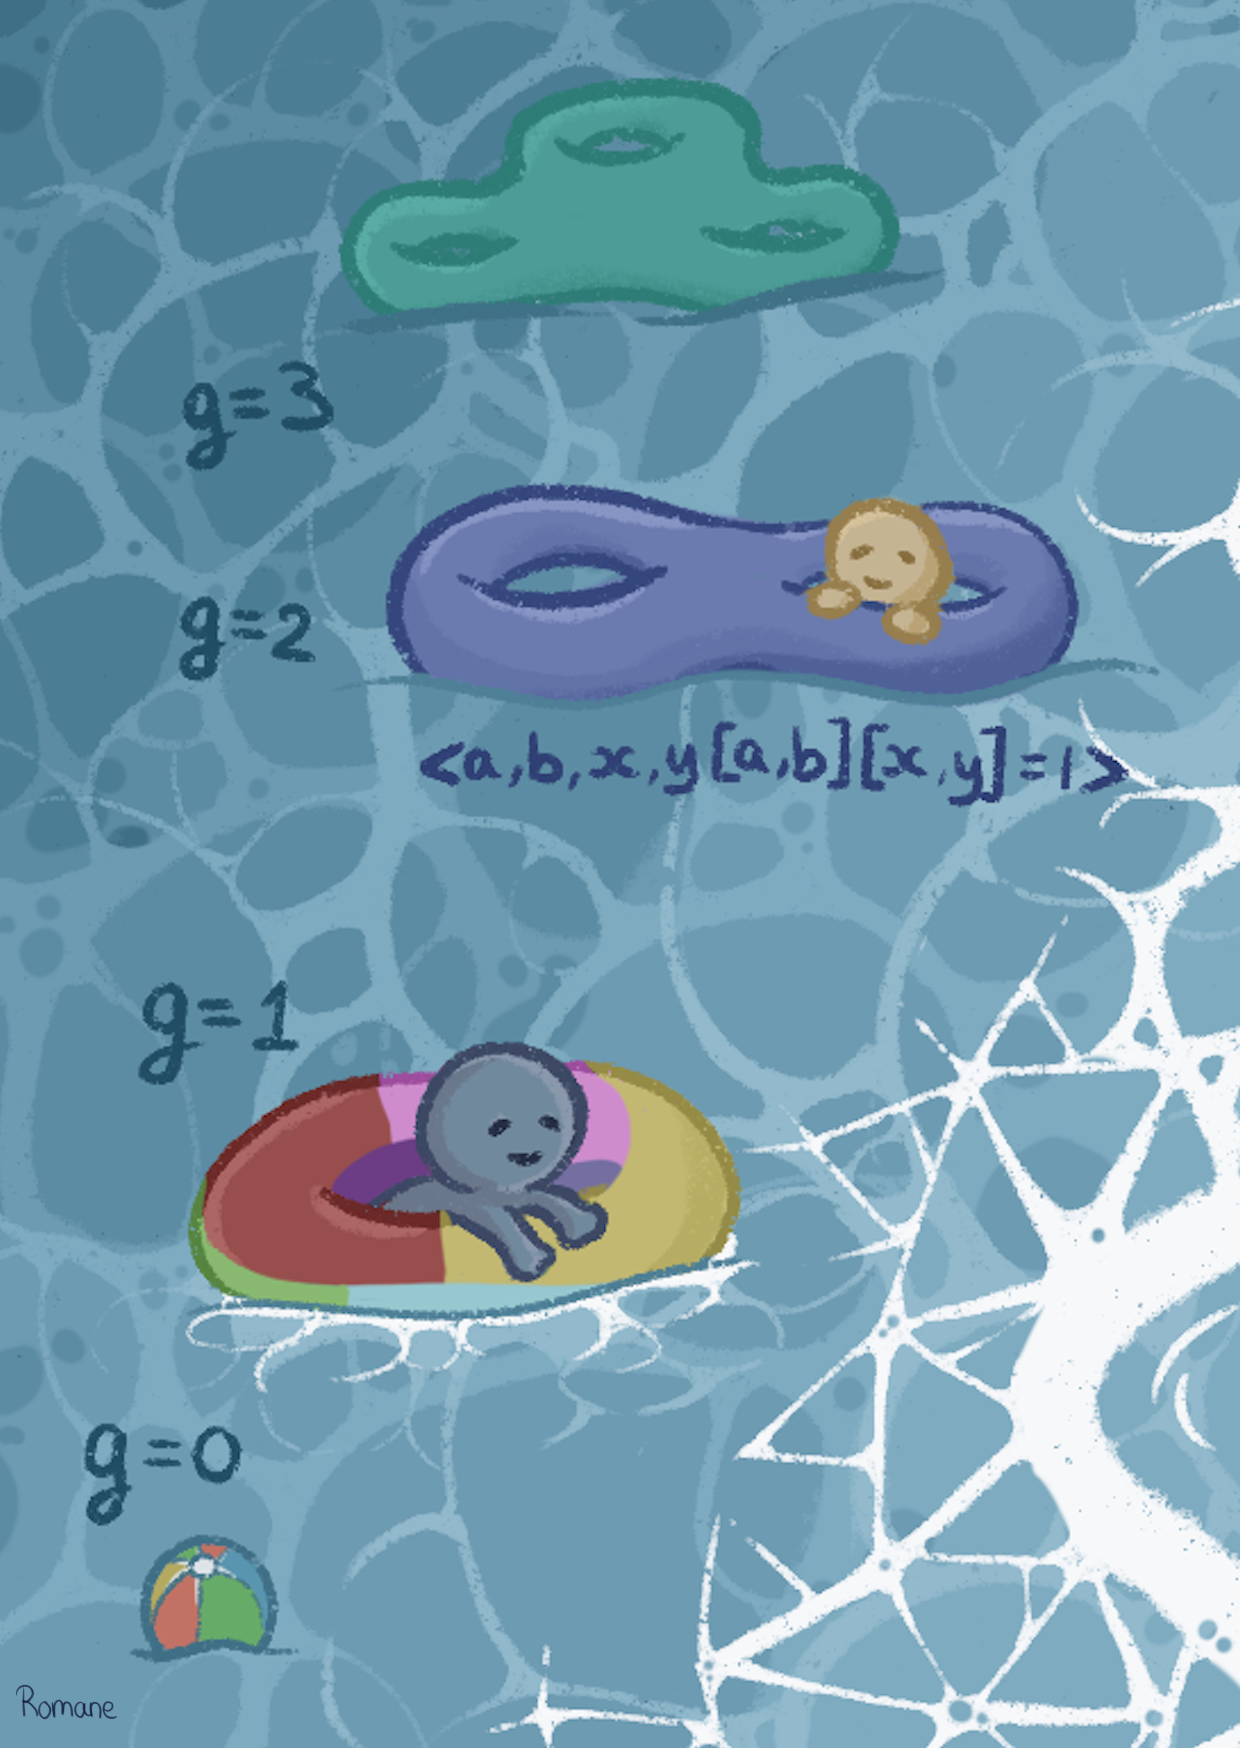
\includegraphics[height=0.5\textheight]{Cartes_postales/carte15-bouee.png}\label{fig:c15}
    \caption{Carte postale: Bouee}
\end{figure}



    \newpage
\section{Tresse}

\begin{figure}[h]
    \centering
    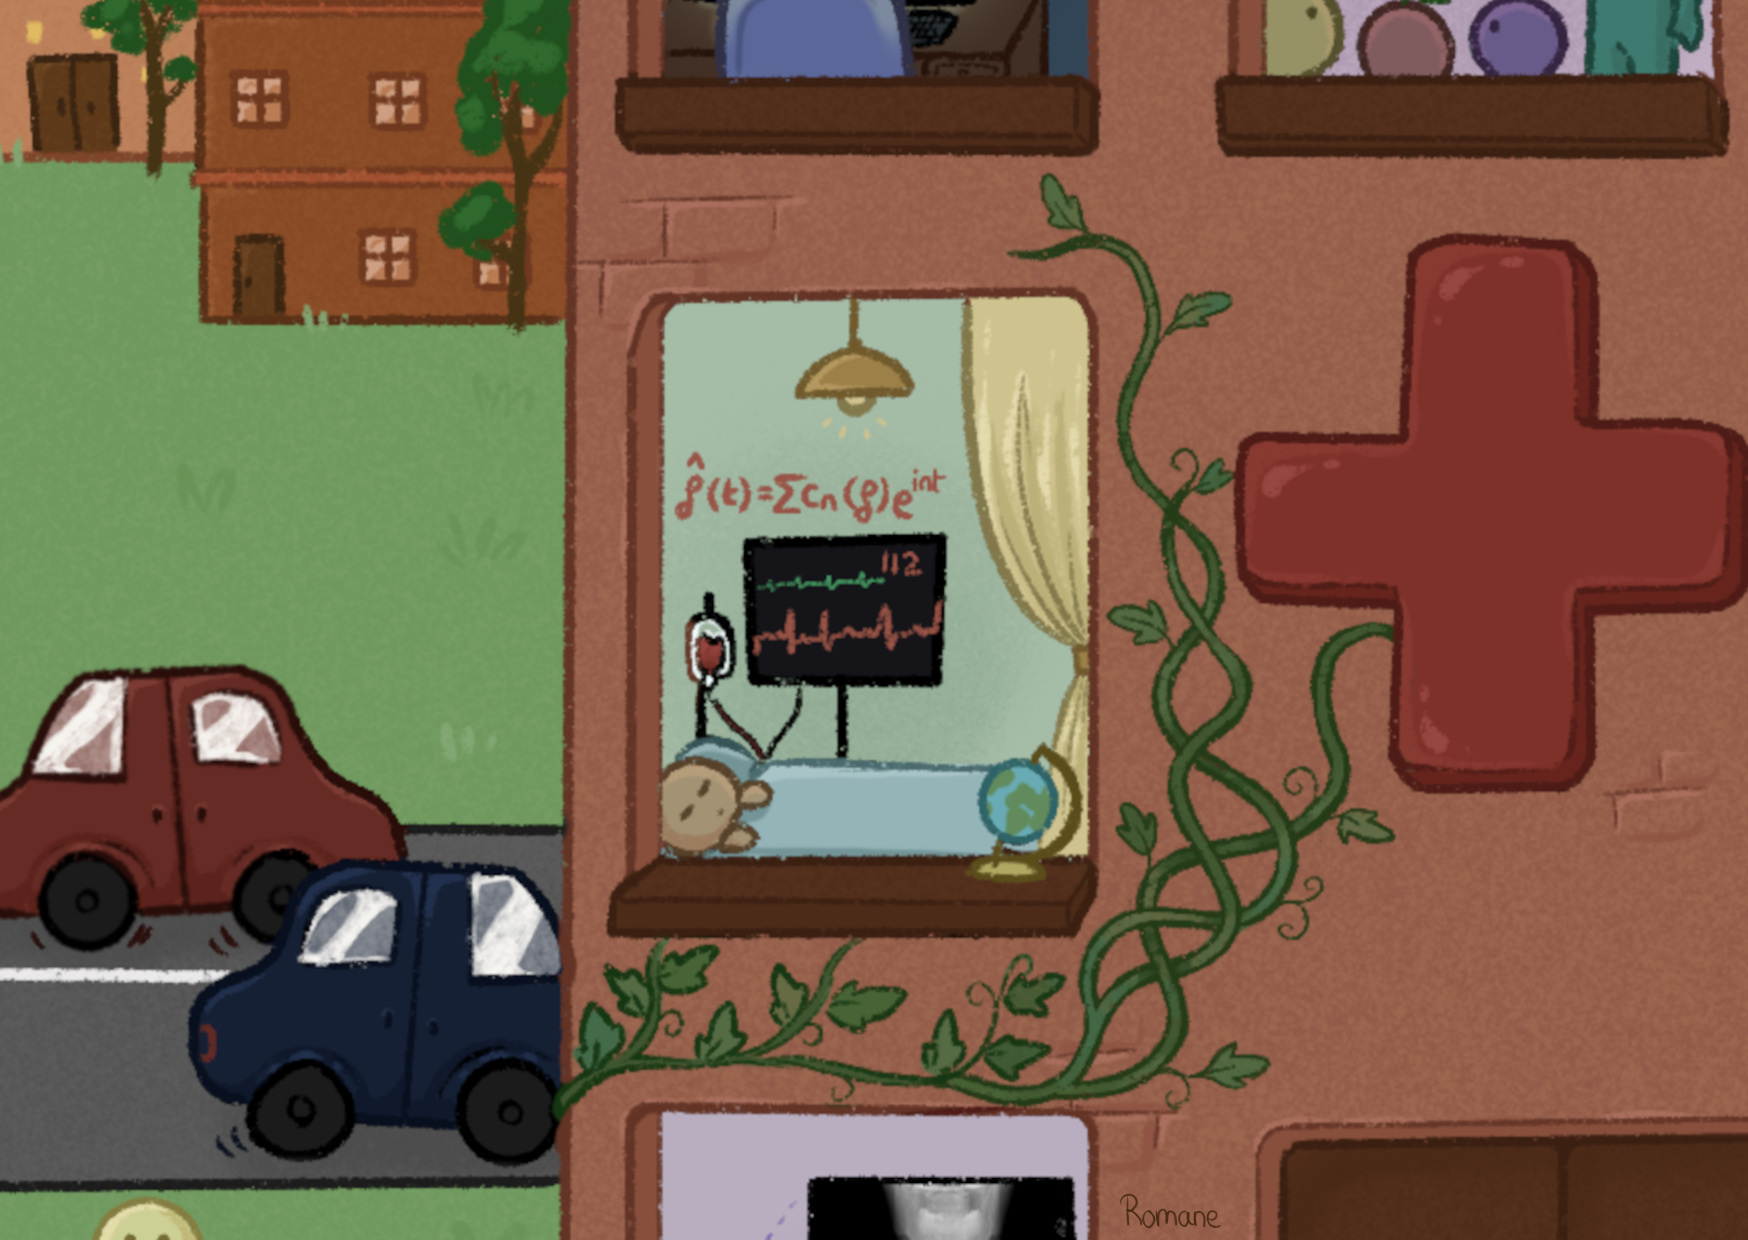
\includegraphics[height=0.5\textheight]{Cartes_postales/carte16-tresse.png}\label{fig:c16}
    \caption{Carte postale: Tresse}
\end{figure}


    \newpage
\section{Binaire}

\begin{figure}[h]
    \centering
    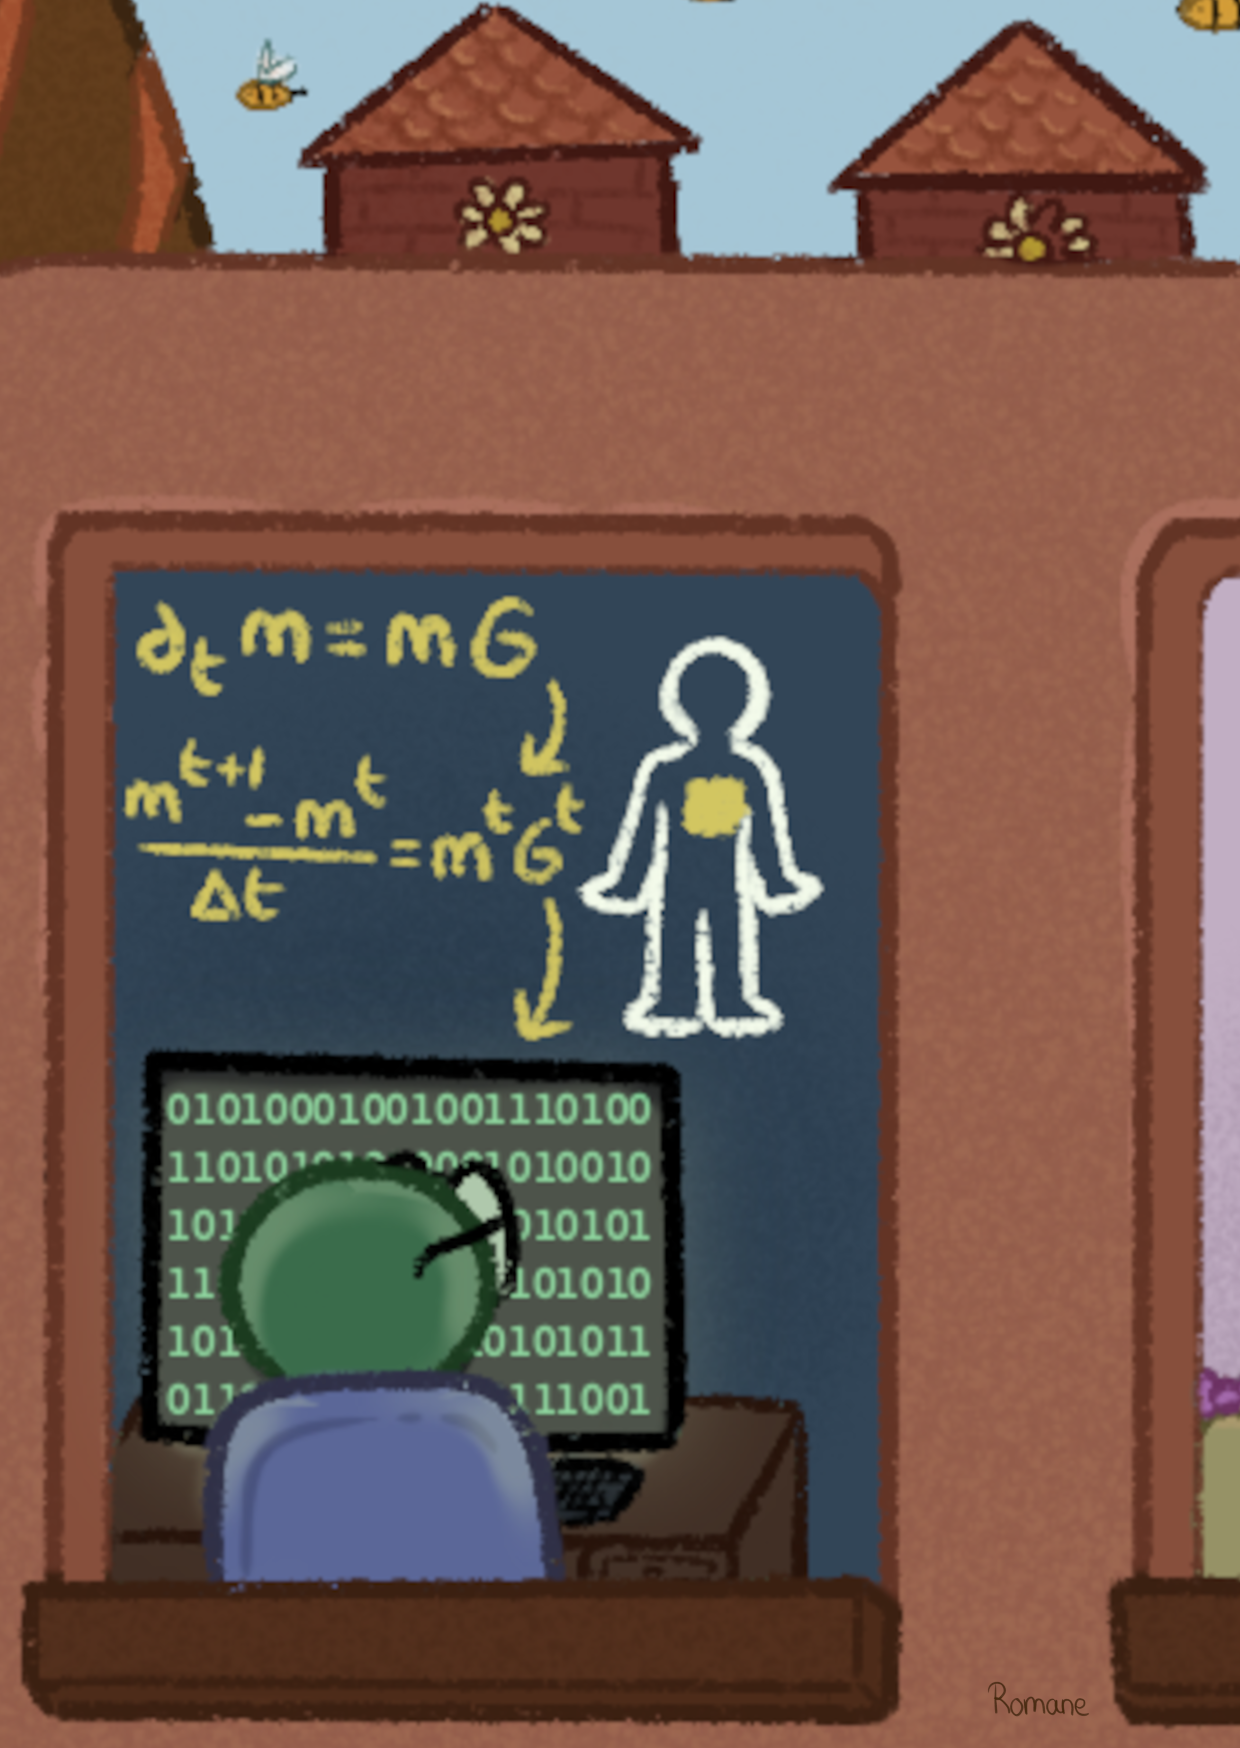
\includegraphics[height=0.5\textheight]{Cartes_postales/carte17-binaire.png}\label{fig:c17}
    \caption{Carte postale: Binaire}
\end{figure}



    \newpage
\section{Neuroscience}

\begin{figure}[h]
    \centering
    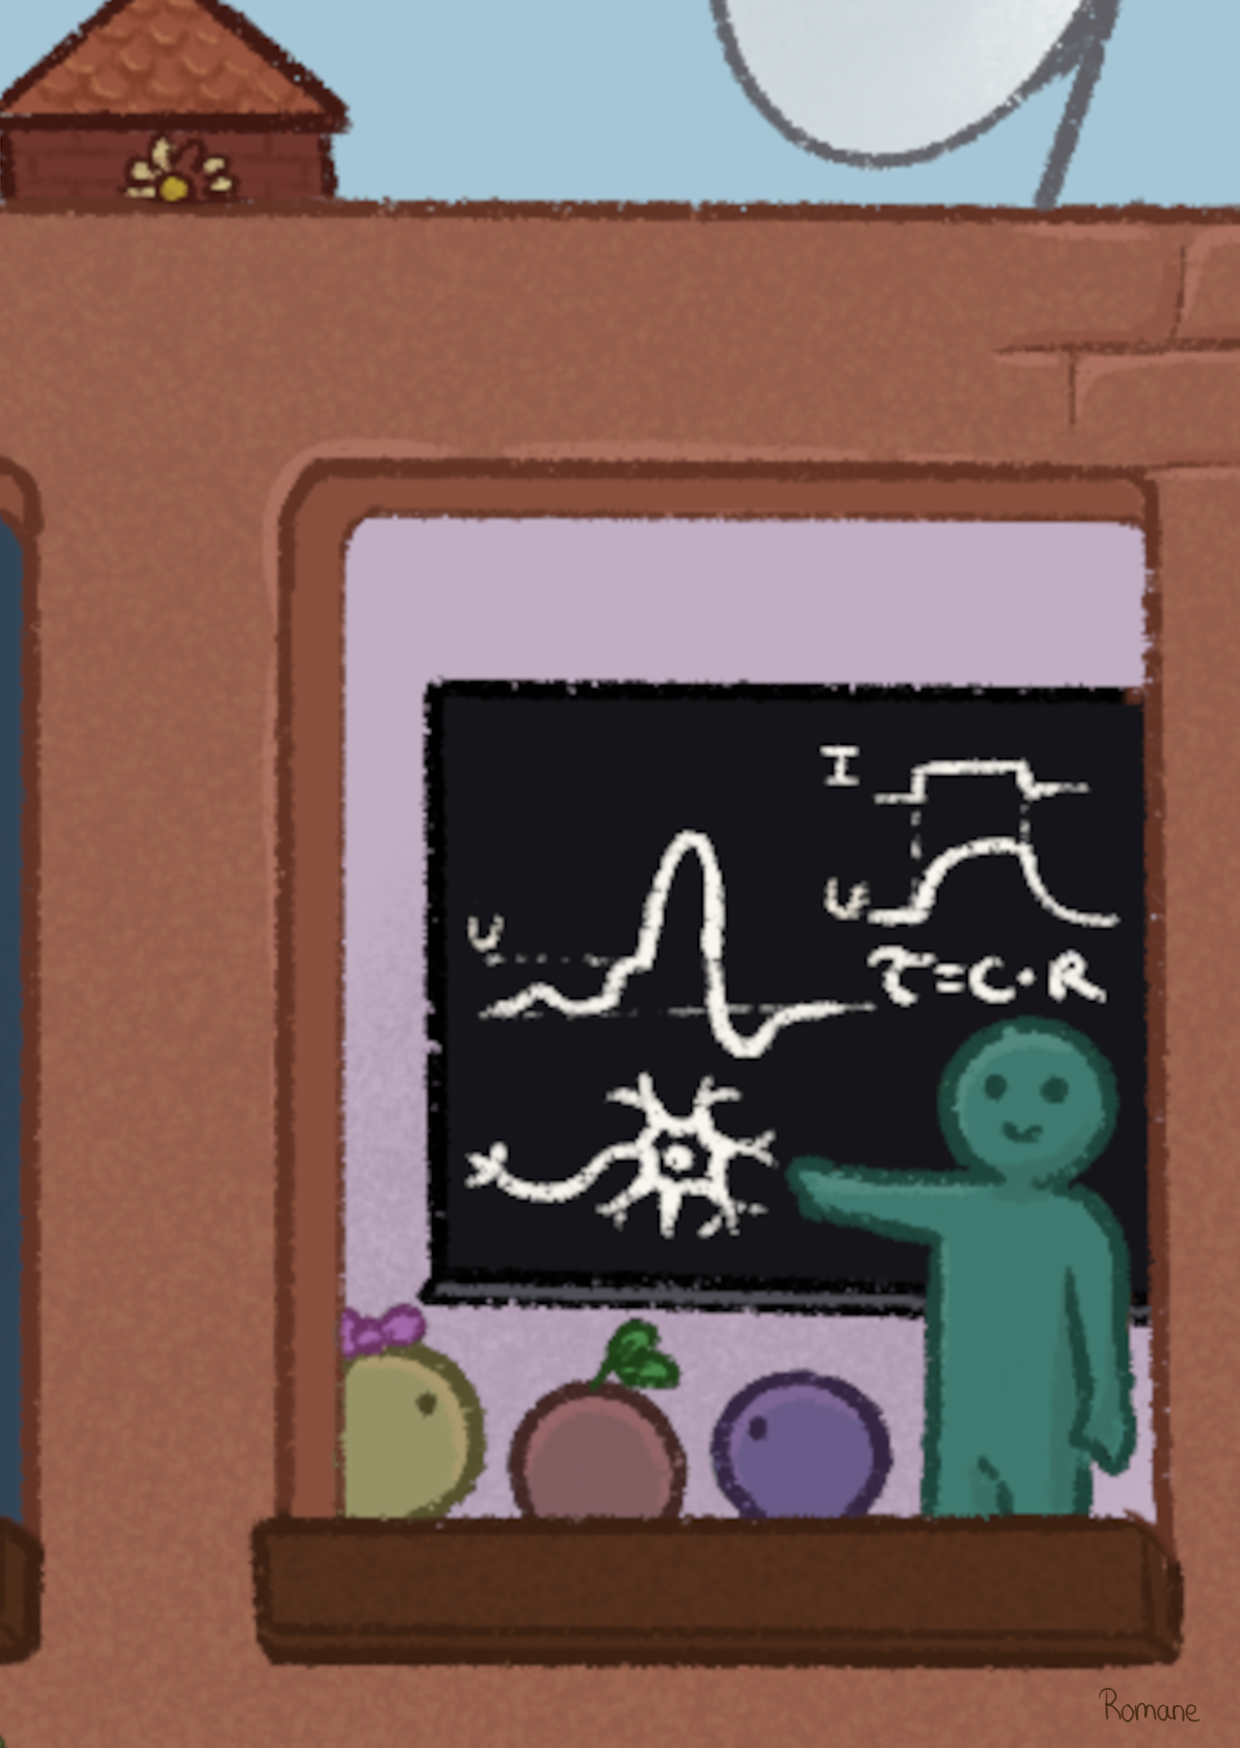
\includegraphics[height=0.5\textheight]{Cartes_postales/carte18-neuroscience.png}\label{fig:c18}
    \caption{Carte postale: Neuroscience}
\end{figure}

    \newpage
\section{Plage}

\begin{figure}[h]
    \centering
    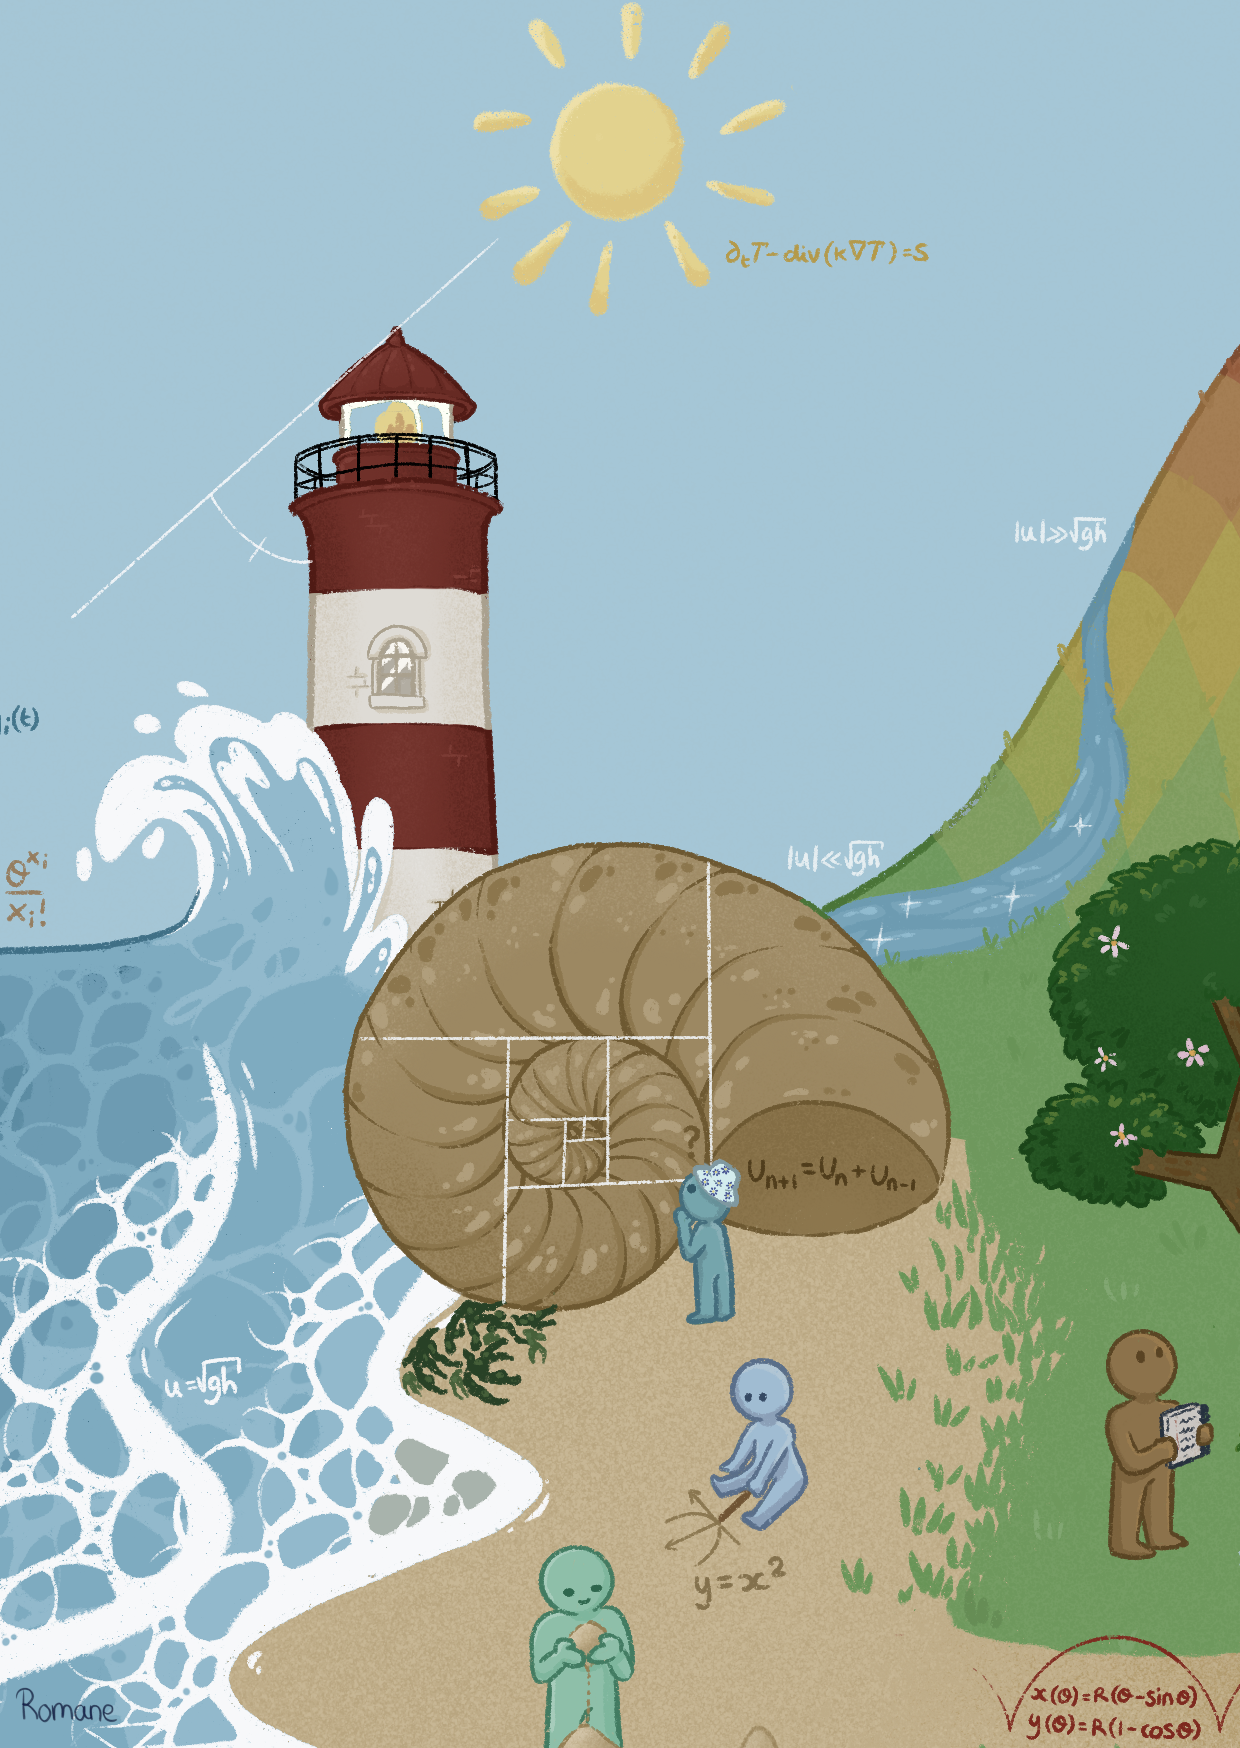
\includegraphics[height=0.5\textheight]{Cartes_postales/carte19-plage.png} 
    \label{fig:mon_image}
    \caption{Carte postale: Plage}
\end{figure}


    \newpage
\section{Mer}

\begin{figure}[h]
    \centering
    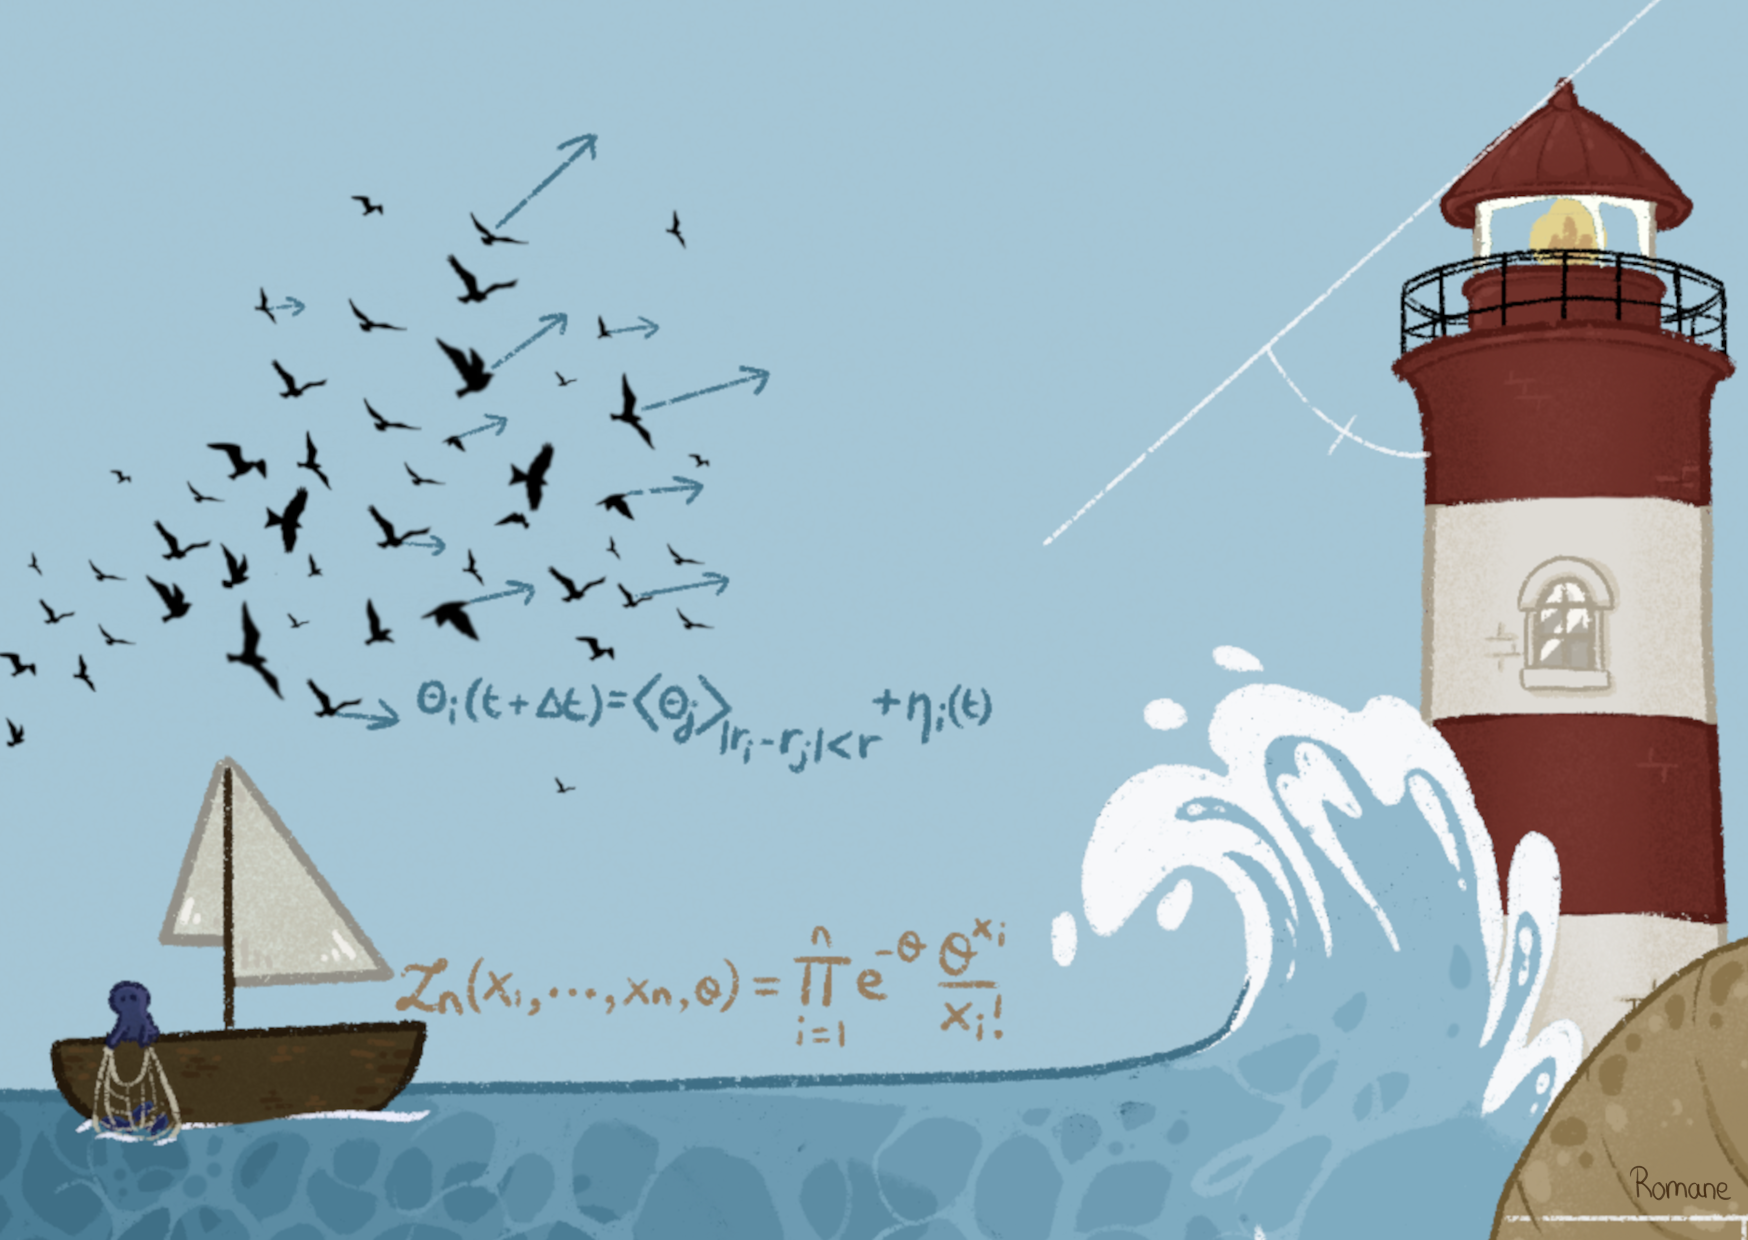
\includegraphics[height=0.5\textheight]{Cartes_postales/carte20-mer.png}\label{fig:c20}
    \caption{Carte postale: Mer}
\end{figure}



    \newpage
\section{Prairie}

\begin{figure}[h]
    \centering
    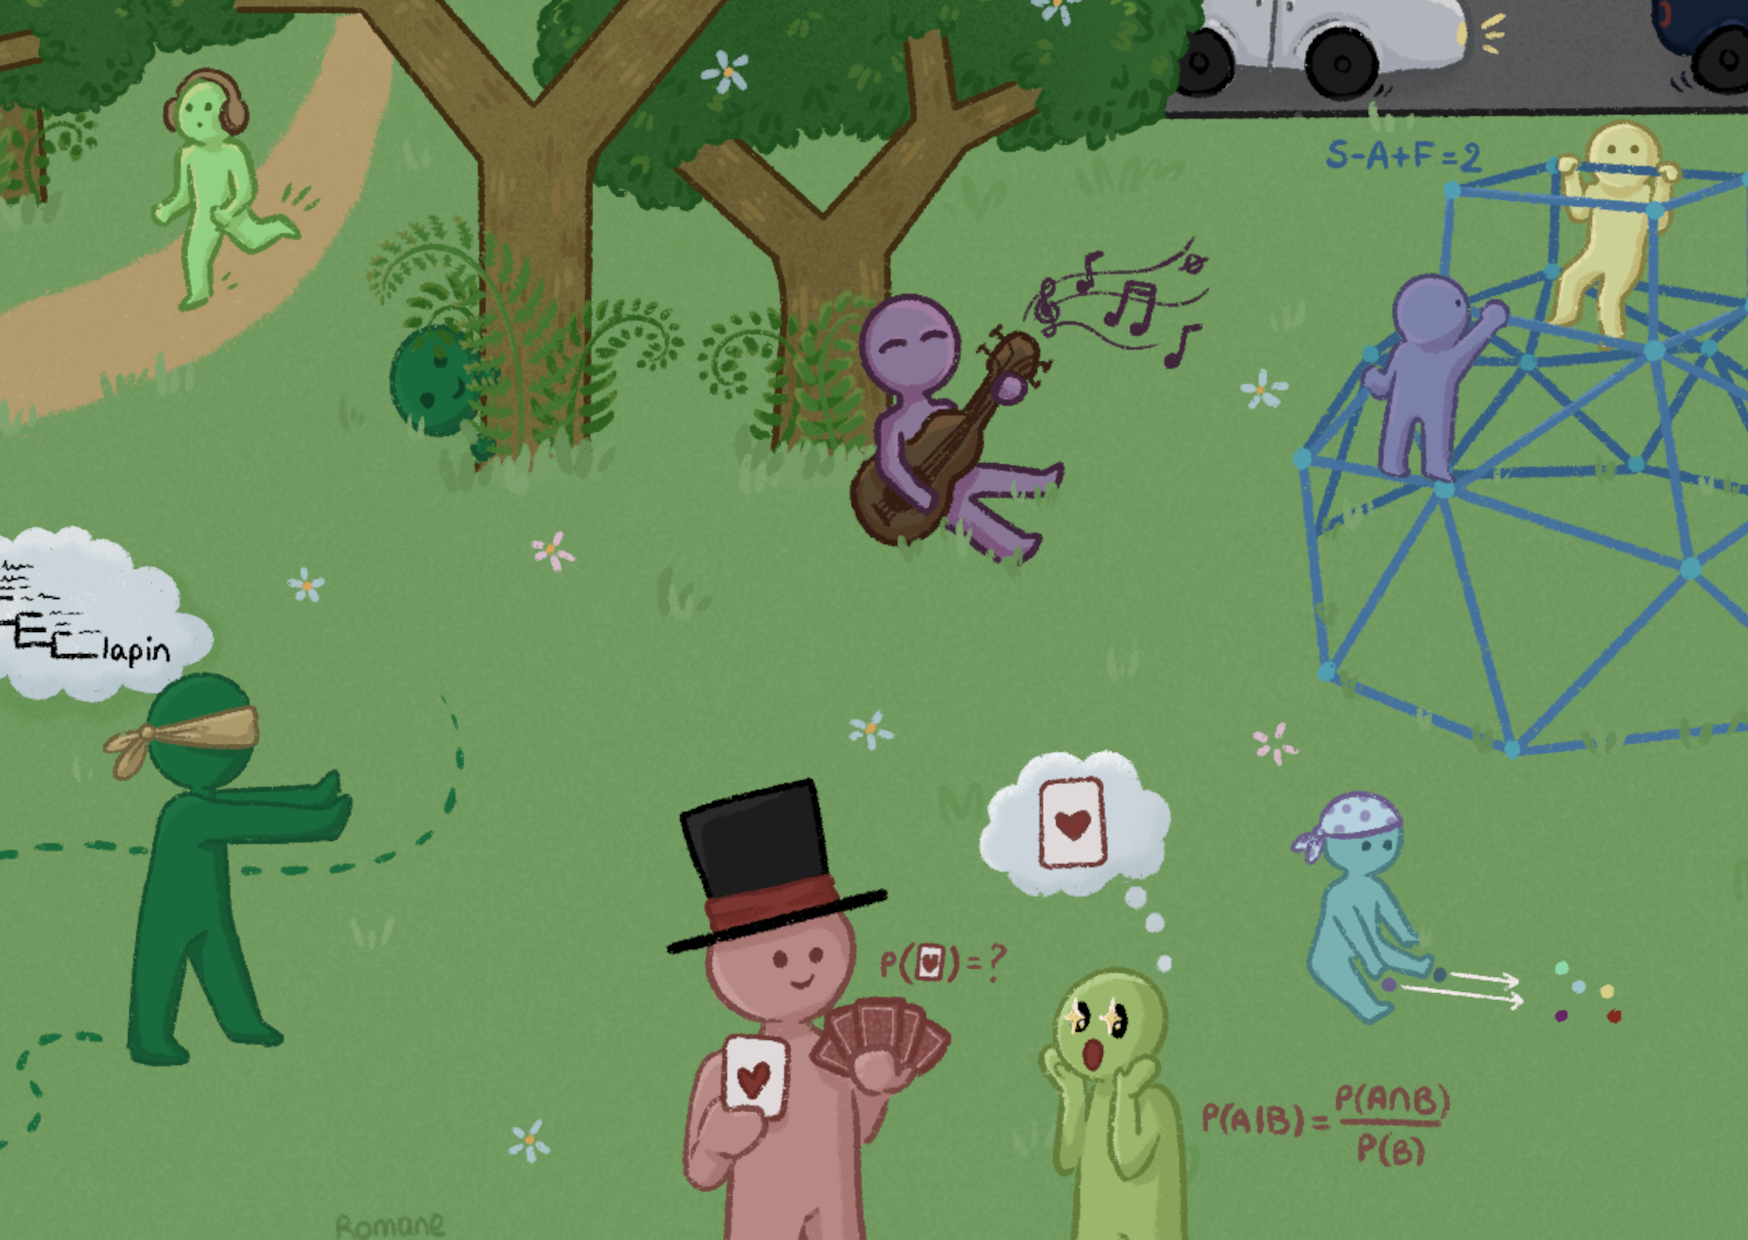
\includegraphics[height=0.5\textheight]{Cartes_postales/carte21-prairie.png} 
    \label{fig:mon_image}
    \caption{Carte postale: Prairie}
\end{figure}


    \newpage
\section{Hopital}

\begin{figure}[h]
    \centering
    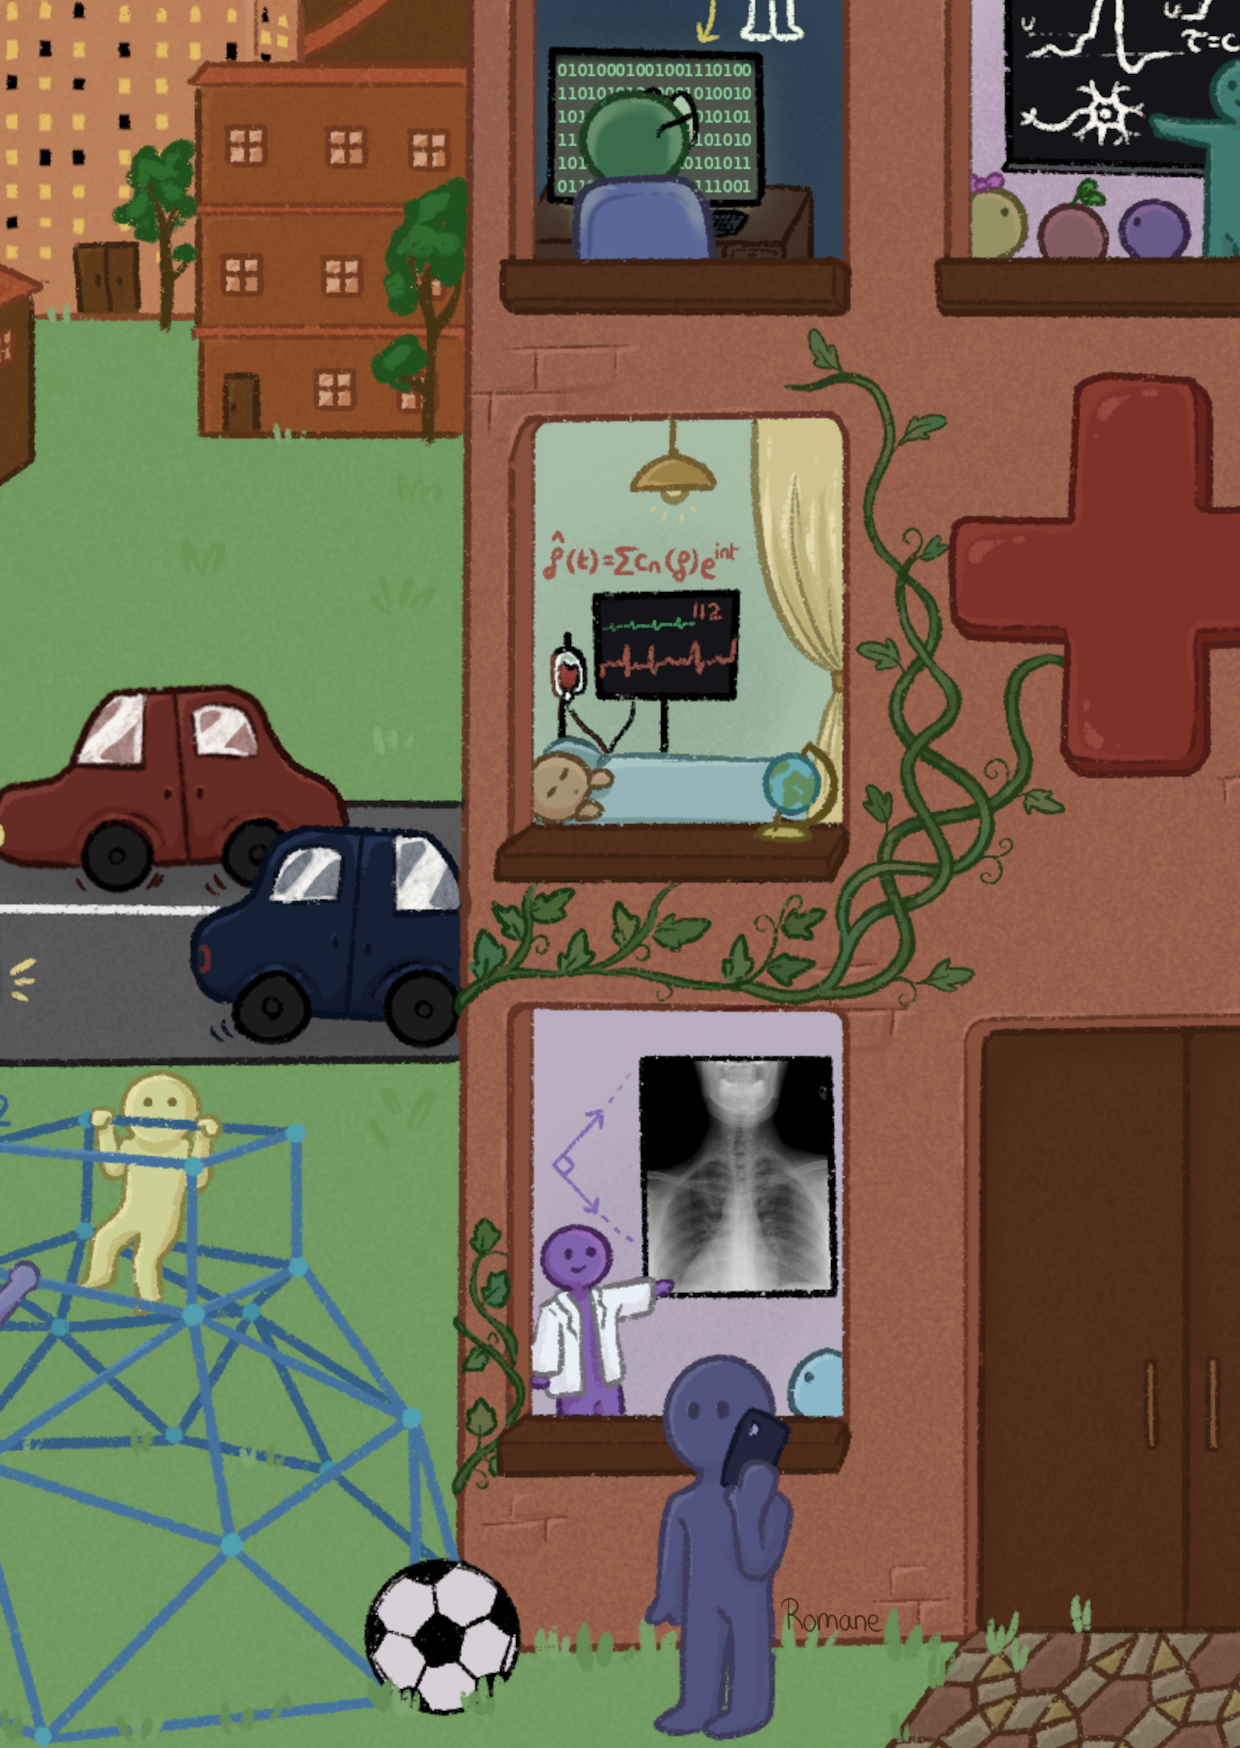
\includegraphics[height=0.5\textheight]{Cartes_postales/carte22-hopital.png}\label{fig:c22}
    \caption{Carte postale: Hopital}
\end{figure}


    \newpage
\section{Forêt}

\begin{figure}[h]
    \centering
    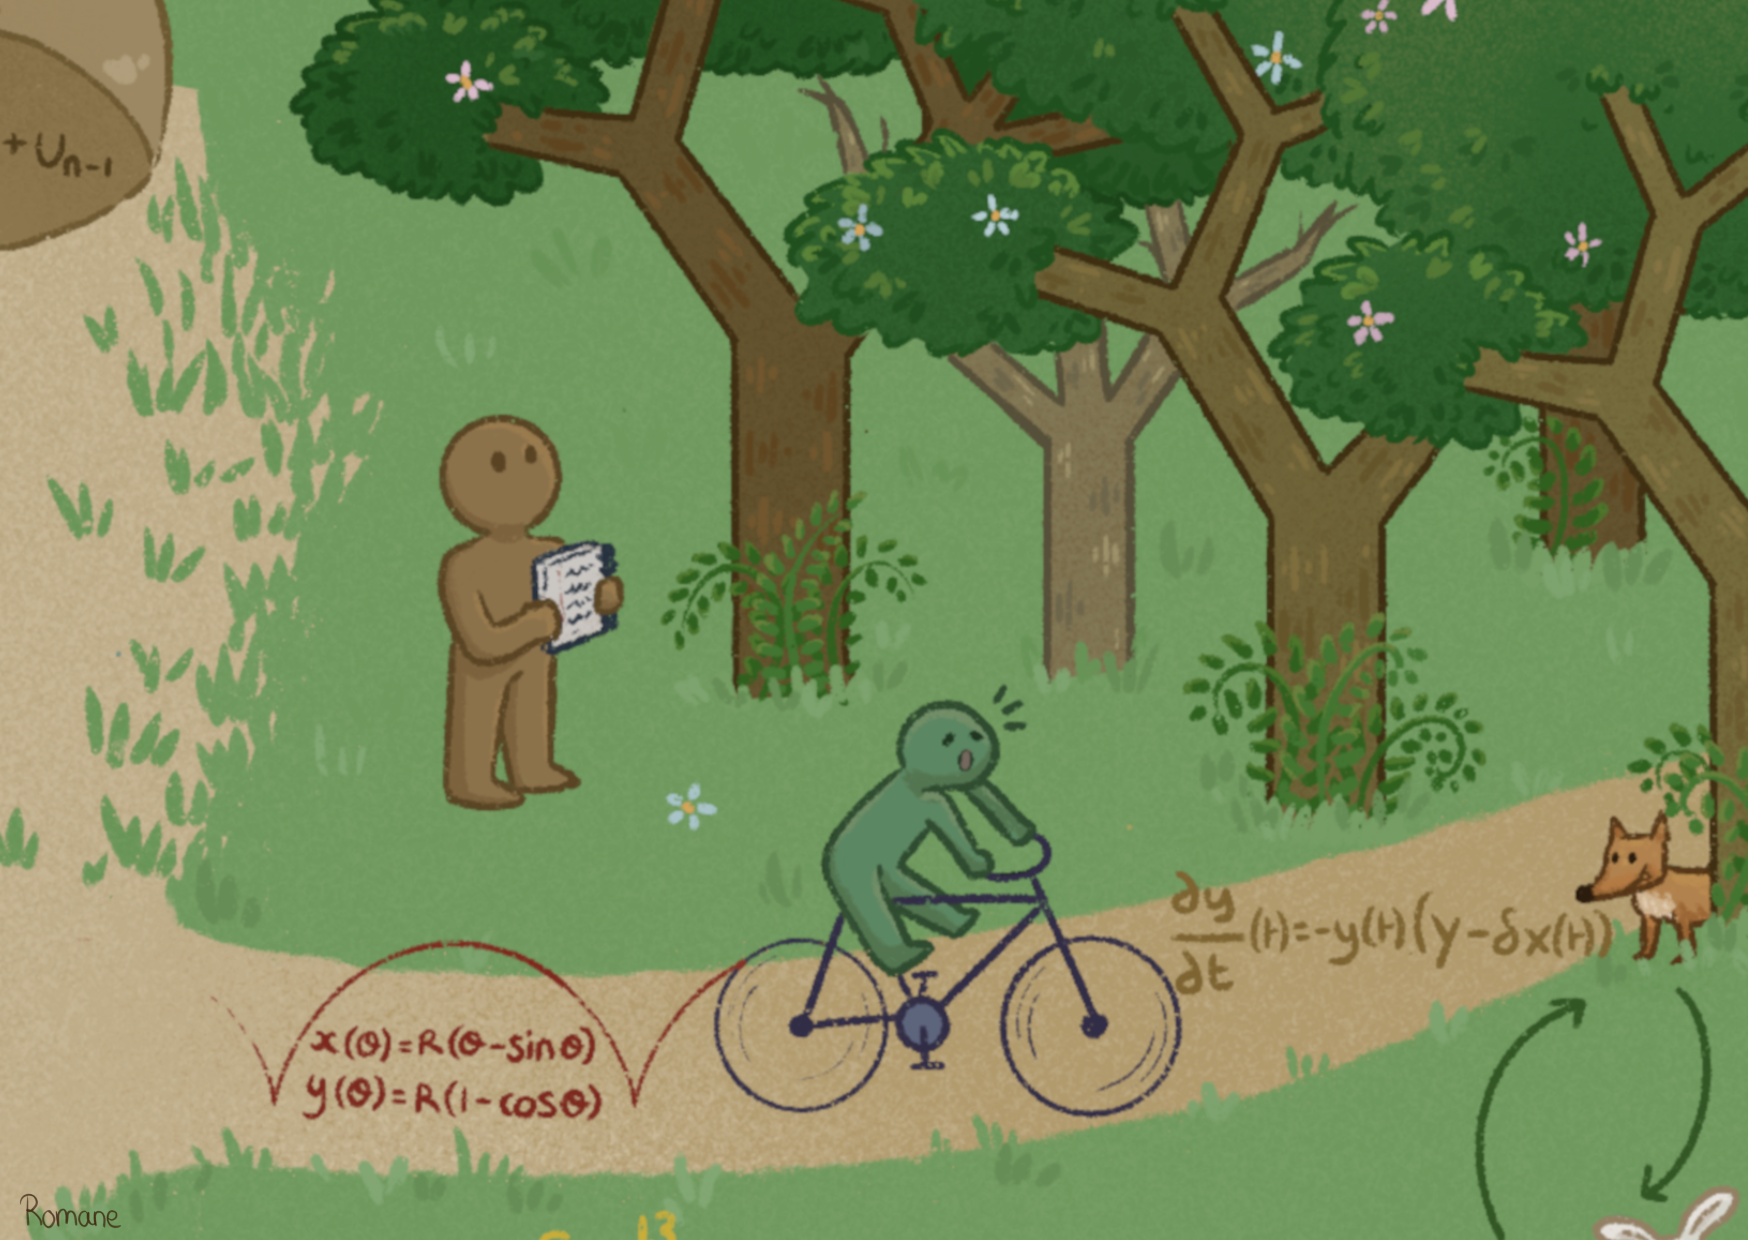
\includegraphics[height=0.5\textheight]{Cartes_postales/carte23-foret.png} 
    \label{fig:mon_image}
    \caption{Carte postale: Forêt}
\end{figure}


    \newpage
\section{Radio}

\begin{figure}[h]
    \centering
    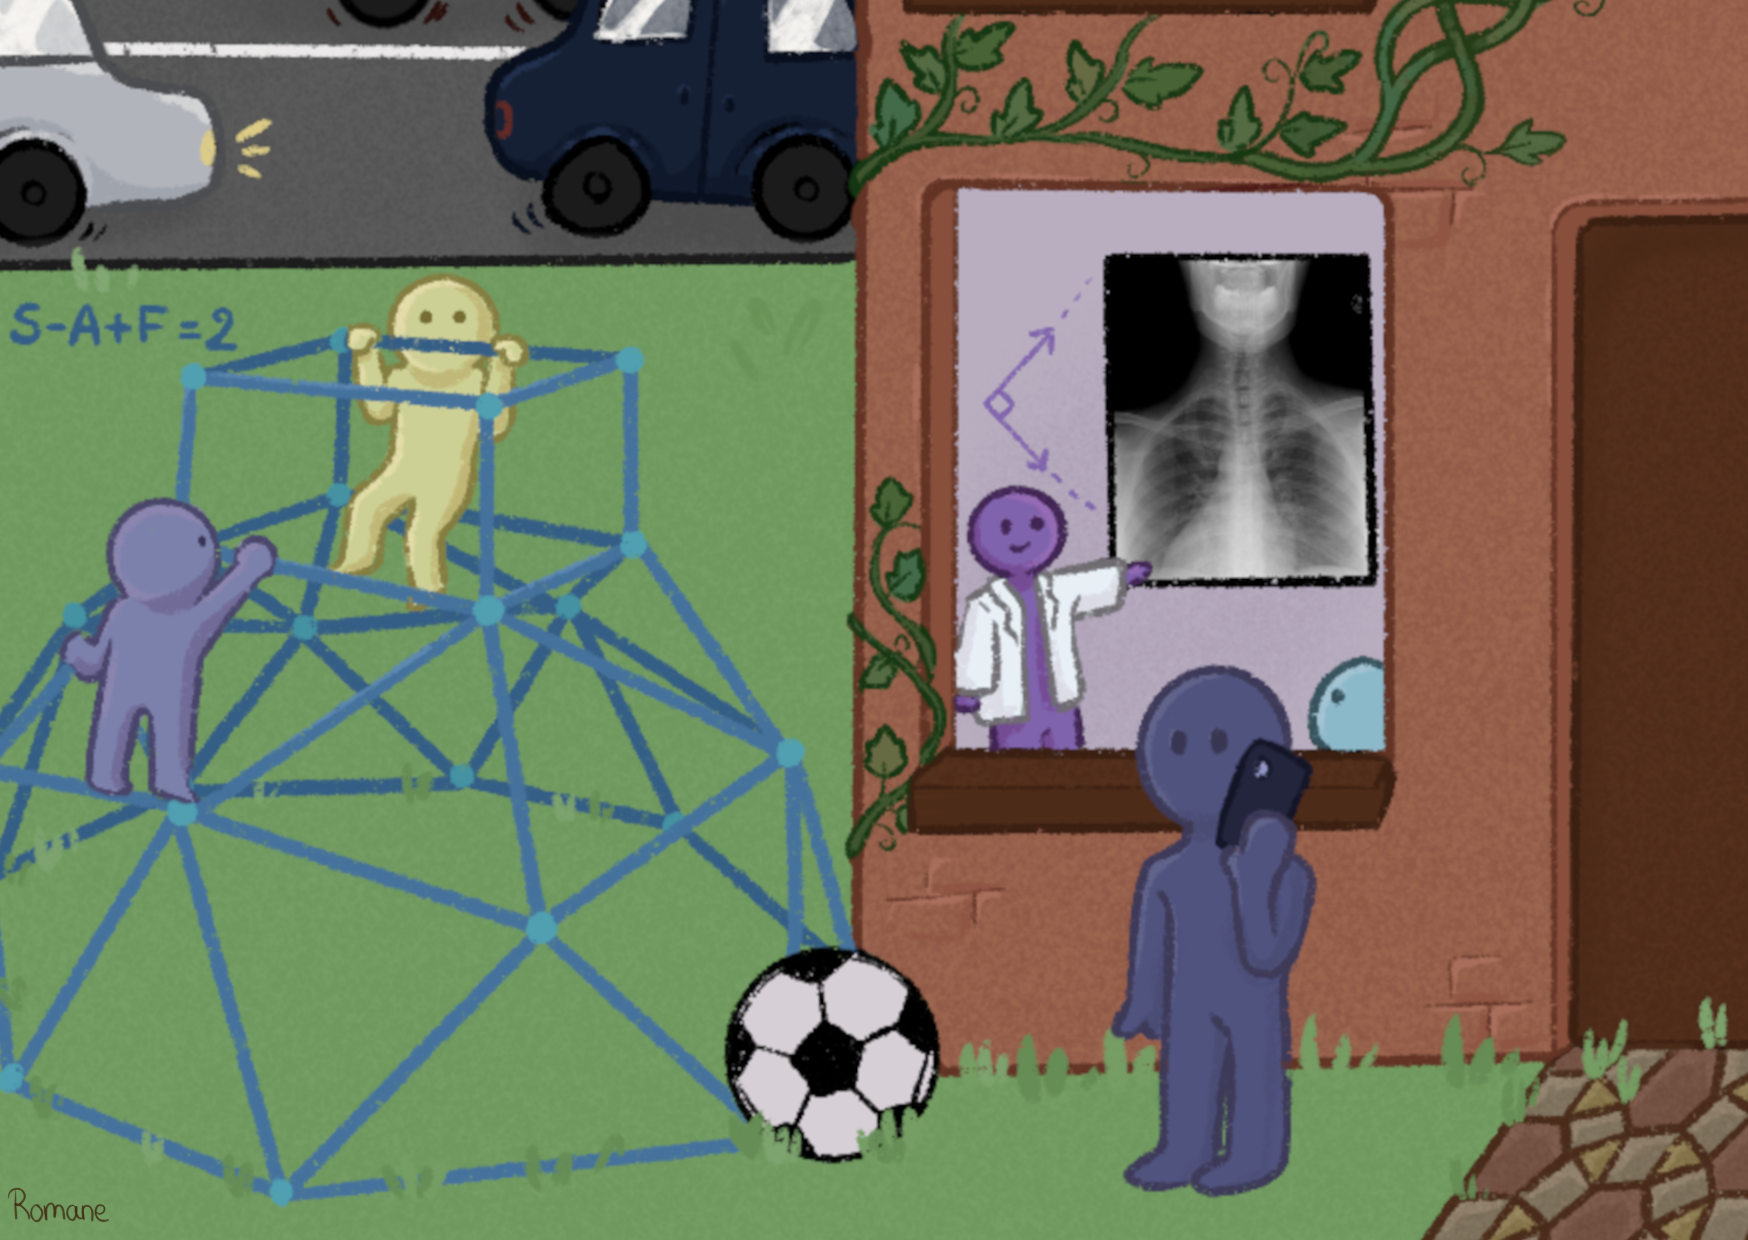
\includegraphics[height=0.5\textheight]{Cartes_postales/carte24-radio.png} 
    \label{fig:mon_image}
    \caption{Carte postale: Radio}
\end{figure}


    

    % \newpage
\end{document}

